\documentclass[a4paper,UKenglish]{lipics-v2018}
%DIF LATEXDIFF DIFFERENCE FILE
%DIF DEL giscience2018_origional.tex   Sun May 27 21:45:20 2018
%DIF ADD giscience2018.tex             Thu May 31 00:46:07 2018
%This is a template for producing LIPIcs articles. 
%See lipics-manual.pdf for further information.
%for A4 paper format use option "a4paper", for US-letter use option "letterpaper"
%for british hyphenation rules use option "UKenglish", for american hyphenation rules use option "USenglish"
% for section-numbered lemmas etc., use "numberwithinsect"
 
\usepackage{microtype}%if unwanted, comment out or use option "draft"

%\graphicspath{{./graphics/}}%helpful if your graphic files are in another directory

%My packages
%\usepackage{amsthm}

%\theoremstyle{definition}
%\newtheorem{definition}{Definition}[section]

%\nolinenumbers
\bibliographystyle{plainurl}% the recommended bibstyle

% Author macros::begin %%%%%%%%%%%%%%%%%%%%%%%%%%%%%%%%%%%%%%%%%%%%%%%%
%\title{Robust Estimation and Comparison of Origin-Destination Flows with Data Depth}\footnote{A full version of the paper is available at \cite{DBLP:journals/cacm/Knuth74}, \url{XXX}}}
\title{Outlier Detection and Comparison of Origin-Destination Flows using Data Depth}
\titlerunning{Outlier Detection and Comparison of Origin-Destination Flows using Data Depth} %optional, in case that the title is too long; the running title should fit into the top page column

%% Please provide for each author the \author and \affil macro, even when authors have the same affiliation, i.e. for each author there needs to be the  \author and \affil macros
\author{Myeong-Hun Jeong}{Department of Civil Engineering, Chosun University, Gwangju, Republic of Korea}{mhjeong@chosun.ac.kr}{[orcid]}{[funding]}
%DIF 28c28
%DIF < \author{Junjun Yin}{Social Science Research Institute; Institute for CyberScience, Penn State University, PA, USA}{jyin@psu.edu}{[orcid]}{[funding]}
%DIF -------
\author{Junjun Yin}{Social Science Research Institute; Institute for CyberScience, Penn State University, PA, USA}{jyin@psu.edu}{[0000-0002-4196-2439]}{[This work used the Extreme Science and Engineering Discovery Environment (XSEDE), which is supported by National Science Foundation grant number ACI-1548562]} %DIF > 
%DIF -------
\author{Shaowen Wang}{Department of Geography and Geographic Information Science, University of Illinois at Urbana-Champaign, IL, USA}{shaowen@illinois.edu}{[orcid]}{[funding]}

\authorrunning{M.-H. Jeong, J. Yin and S. Wang} %mandatory. First: Use abbreviated first/middle names. Second (only in severe cases): Use first author plus 'et. al.'

\Copyright{Myeong-Hun Jeong, Junjun Yin, and Shaowen Wang}%mandatory, please use full first names. LIPIcs license is "CC-BY";  http://creativecommons.org/licenses/by/3.0/

%\subjclass{Dummy classification -- please refer to \url{http://www.acm.org/about/class/ccs98-html}}% mandatory: Please choose ACM 1998 classifications from http://www.acm.org/about/class/ccs98-html . E.g., cite as "F.1.1 Models of Computation". 

\subjclass{Computing methodologies $\rightarrow$ Anomaly detection}% mandatory: Please choose ACM 2012 classifications from https://www.acm.org/publications/class-2012 or https://dl.acm.org/ccs/ccs_flat.cfm . E.g., cite as "General and reference $\rightarrow$ General literature" or \ccsdesc[100]{General and reference~General literature}.

\keywords{OD Analysis, Trajectory Data Mining, Data Depth, Outliers Detection}% mandatory: Please provide 1-5 keywords

\category{}%optional, e.g. invited paper

\relatedversion{}%optional, e.g. full version hosted on arXiv, HAL, or other respository/website

\supplement{}%optional, e.g. related research data, source code, ... hosted on a repository like zenodo, figshare, GitHub, ...

\funding{}%optional, to capture a funding statement, which applies to all authors. Please enter author specific funding statements as fifth argument of the \author macro.

\acknowledgements{I want to thank \dots}%optional
% Author macros::end %%%%%%%%%%%%%%%%%%%%%%%%%%%%%%%%%%%%%%%%%%%%%%%%%

%Editor-only macros:: begin (do not touch as author)%%%%%%%%%%%%%%%%%%%%%%%%%%%%%%%%%%
\EventEditors{Stephan Winter, Amy Griffin, and Monika Sester}
\EventNoEds{3}
\EventLongTitle{10th International Conference on Geographic Information Science (GIScience 2018)}
\EventShortTitle{GIScience 2018}
\EventAcronym{GIScience}
\EventYear{2018}
\EventDate{August 28--31, 2017}
\EventLocation{Melbourne, Australia}
\EventLogo{}
\SeriesVolume{114}
\ArticleNo{6} % “New number” (=<article-no>) goes here!
% Editor-only macros::end %%%%%%%%%%%%%%%%%%%%%%%%%%%%%%%%%%%%%%%%%%%%%%%
%DIF PREAMBLE EXTENSION ADDED BY LATEXDIFF
%DIF UNDERLINE PREAMBLE %DIF PREAMBLE
\RequirePackage[normalem]{ulem} %DIF PREAMBLE
\RequirePackage{color}\definecolor{RED}{rgb}{1,0,0}\definecolor{BLUE}{rgb}{0,0,1} %DIF PREAMBLE
\providecommand{\DIFadd}[1]{{\protect\color{blue}\uwave{#1}}} %DIF PREAMBLE
\providecommand{\DIFdel}[1]{{\protect\color{red}\sout{#1}}}                      %DIF PREAMBLE
%DIF SAFE PREAMBLE %DIF PREAMBLE
\providecommand{\DIFaddbegin}{} %DIF PREAMBLE
\providecommand{\DIFaddend}{} %DIF PREAMBLE
\providecommand{\DIFdelbegin}{} %DIF PREAMBLE
\providecommand{\DIFdelend}{} %DIF PREAMBLE
%DIF FLOATSAFE PREAMBLE %DIF PREAMBLE
\providecommand{\DIFaddFL}[1]{\DIFadd{#1}} %DIF PREAMBLE
\providecommand{\DIFdelFL}[1]{\DIFdel{#1}} %DIF PREAMBLE
\providecommand{\DIFaddbeginFL}{} %DIF PREAMBLE
\providecommand{\DIFaddendFL}{} %DIF PREAMBLE
\providecommand{\DIFdelbeginFL}{} %DIF PREAMBLE
\providecommand{\DIFdelendFL}{} %DIF PREAMBLE
%DIF END PREAMBLE EXTENSION ADDED BY LATEXDIFF

\begin{document}

\maketitle

\begin{abstract}
Advances in location-aware technology have \DIFdelbegin \DIFdel{resulted in }\DIFdelend \DIFaddbegin \DIFadd{led to }\DIFaddend the generation of a huge volume of trajectory data.
Origin-destination (OD) trajectories provide rich information on urban flow and transport demand.
This study presents a new methodology to detect OD \DIFdelbegin \DIFdel{flows }\DIFdelend \DIFaddbegin \DIFadd{flow }\DIFaddend outliers and conduct hypothesis testing between two OD flows in terms of the variations of spatial extent, \DIFdelbegin \DIFdel{that is}\DIFdelend \DIFaddbegin \DIFadd{namely}\DIFaddend , spread.
The proposed method is based on data depth, which measures the centrality and outlyingness of a point with respect to a given dataset in $\mathbb{R}^d$.
Based on the center-outward ordering property, the proposed method analyzes the underlying characteristics of OD flows, such as location, outlyingness, and spread.
The ability of the proposed method to detect OD anomalies is compared with that of the Mahalanobis distance approach, and an F-test is used to verify the difference in scale. Empirical evaluation has demonstrated that the proposed method effectively identifies OD flows outliers in an interactive way. Furthermore, the proposed method can provide new perspectives by considering the overall structure of data when comparing two different OD flows in terms of scale. 

 \end{abstract}

\section{Introduction}
With the rapid rise in ubiquity of geolocation-aware sensors, knowledge discovery is greatly enhanced by extracting and mining interesting patterns from spatiotemporal big data in various domains.
Location-acquisition technologies generate large volumes of movement data, which are used to track people, animals, vehicles, and even natural phenomena.
Such data help us better model moving objects and reveal hidden patterns that are important to urban planning \cite{mazimpaka15AGILE}, urban human mobility \cite{yin2017depicting,kwan1998space}, the sustainability of urban systems \cite{alberti2003integrating,chen13Percom}, the environment \cite{devarakonda13SIGKDD}, and public security and safety \cite{buchin14JOSIS}.
%DIF < Importantly, trajectory mining leads to solutions for addressing important research problems in different fields, such as urban planning \cite{mazimpaka15AGILE}, transportation \cite{chen13Percom}, environment \cite{devarakonda13SIGKDD}, and public security and safety \cite{buchin14JOSIS}.

This paper presents a new algorithm which \DIFdelbegin \DIFdel{estimates }\DIFdelend \DIFaddbegin \DIFadd{identifies }\DIFaddend origination-destination (OD) flow anomalies and conducts hypothesis testing between two sets of different OD flows.
In this study, the OD flow data is a subset of trajectory data, which records the origin and destination of each movement while ignoring the \DIFdelbegin \DIFdel{actual }\DIFdelend \DIFaddbegin \DIFadd{exact }\DIFaddend trajectory route \cite{guo14IEEETVCG}.
The algorithm was applied to OD flows derived from \DIFdelbegin \DIFdel{extracted origin and destination data in a dataset describing }\DIFdelend \DIFaddbegin \DIFadd{the }\DIFaddend New York City taxi \DIFdelbegin \DIFdel{trips}\DIFdelend \DIFaddbegin \DIFadd{trip records}\DIFaddend , in which each record contained the origin and destination of each trip \DIFdelbegin \DIFdel{, }\DIFdelend without intermediate locations of the actual routes.

In recent years, researchers have investigated a variety of approaches to trajectory data mining.
Most contemporary trajectory mining methods can be classified into four categories: clustering, classification, frequent/group pattern mining, and outlier detection \cite{mazimpaka16JOSIS,zheng15ACMTIST}.
These techniques can be used independently or combinatorially for trajectory mining applications.
This study focuses on outlier detection of OD flows.
Outlier detection attempts to identify trajectories that do not follow the typical flows of trajectory datasets that characterizes the connectivity between regions \cite{mazimpaka16JOSIS}.
Euclidean distance is employed by \cite{fontes13GeoInfo,lee08ICDE} to find outlier patterns from trajectories.
Studies by \cite{pan13ACMGIS,liu12IJGIS} question the Euclidean distance approach because of the loss of local features and unavailability when external factors, such as topography, land cover or weather condition, \DIFaddbegin \DIFadd{may }\DIFaddend affect the trajectories.
In their research, \cite{pan13ACMGIS,liu12IJGIS} addresses this by using robust distance measurements, i.e., Mahalanobis distance \cite{pan13ACMGIS} and relative distance \cite{liu12IJGIS}.
Instead of using distance or density, anomalous trajectories are detected by exploiting comparisons of the structural features of each trajectory segment \cite{yuan11JCIS} and an isolation tree of trajectories \cite{zhang11UC}.
Most of the above methods are related to trajectory data analysis\DIFdelbegin \DIFdel{, and thus, }\DIFdelend \DIFaddbegin \DIFadd{.
In this connection, }\DIFaddend it is reasonable to extend the application of these approaches to the identification of OD flow anomalies. 
To overcome the sensitivity of Euclidean distance-based approaches to \DIFaddbegin \DIFadd{data with }\DIFaddend non-normal \DIFdelbegin \DIFdel{distributed data }\DIFdelend \DIFaddbegin \DIFadd{distributions }\DIFaddend and the difficulty of selecting parameters for anomaly detection techniques based on distance or density, this study employs robust statistics, \DIFdelbegin \DIFdel{such as }\DIFdelend \DIFaddbegin \DIFadd{specifically }\DIFaddend data depth, to detect OD flow outliers.

%DIF <  Although most methods mentioned above are related to trajectory data analysis, it is reasonable to extend these approaches to identify  OD flows anomaly. Thus, this study employs robust statistics such as data depth to detect robustly OD flow outliers because Euclidean distance-based approaches are sensitive to non-normal distributed data and it is hard to choose  parameters for anomaly detection techniques based on distance or density.   
%DIF <   because  Euclidean distance-based approaches are sensitive to non-normal distribution of data sets. 
\DIFdelbegin %DIFDELCMD < 

%DIFDELCMD < %%%
%DIF < In a similar fashion, this study considers the center regions of OD flows with data depth in order to robustly detect the OD flows outliers. 
%DIFDELCMD < 

%DIFDELCMD < %%%
%DIF < In addition, visual analytics such as flow mapping is a common approach to analyze OD flow data. Visual representations of massive movement data enables comprehensive exploration of data and results in understanding complex flow trends.
%DIFDELCMD < 

%DIFDELCMD < %%%
\DIFdelend Flow mapping, \DIFaddbegin \DIFadd{as }\DIFaddend a type of visual analytics, is a common approach to analyzing OD flow data.
Visual representations of massive movement data facilitate comprehensive exploration of data, in turn enabling perception and understanding complex flow trends.
Aggregation and generalization of movement data are frequently utilized to resolve visual clutter \DIFdelbegin \DIFdel{\mbox{%DIFAUXCMD
\cite{guo14IEEETVCG}}%DIFAUXCMD
.
%DIF < \cite{andrienko08VAST,adrienko11IEEETVCG,guo14IEEETVCG}
}\DIFdelend \DIFaddbegin \DIFadd{\mbox{%DIFAUXCMD
\cite{guo14IEEETVCG,yin2016exploring}}%DIFAUXCMD
.
}\DIFaddend While visual analytics can help to extract inherent patterns from massive data, it is difficult to quantitatively compare two sets of different OD flows based on a hypothesis testing.
In other words, it is complicated to comprehend how two OD flows differ and, more importantly, the magnitude of the difference, using a test of statistical significance.
Recently \DIFdelbegin \DIFdel{published articles }\DIFdelend \DIFaddbegin \DIFadd{literatures }\DIFaddend employ multidimensional spatial scan statistics \cite{Gao17IJGIS} and local Ripley’s K-function \cite{tao16GA} to identify clusters of flow data based on statistical significance tests.
\DIFdelbegin \DIFdel{Thus, this }\DIFdelend \DIFaddbegin \DIFadd{This }\DIFaddend paper applies bivariate hypothesis testing methods based on data depth to understand the difference between two OD flow datasets in terms of the amount of spatial extent. 

It is worth noting that flow mapping approaches frequently suffer from the modifiable areal unit problem (MAUP). 
Essentially, MAUP is the influence of different aggregations determined by location on the presentation of coherent patterns.
Kernel-based flow estimation and smoothing are used to overcome different spatial resolutions \cite{guo14IEEETVCG}. 
Instead of attempting to find the best areal unit by which to partition urban space and aggregates the OD flows, this study adopted the established traffic analysis zones of New York City as \DIFdelbegin \DIFdel{base unit}\DIFdelend \DIFaddbegin \DIFadd{the base units}\DIFaddend .
That said, the proposed method can be adapted to other implementation of areal units.
In this study, New York City taxi trip data \DIFdelbegin \DIFdel{includes }\DIFdelend \DIFaddbegin \DIFadd{include }\DIFaddend the origin and destination within traffic analysis zones, while ignoring the intermediate locations of the actual routes.
\DIFdelbegin \DIFdel{It }\DIFdelend \DIFaddbegin \DIFadd{Note that it }\DIFaddend is not necessary to reconstruct individual movements for flow estimation (see \cite{duckham16ICGIS}).

In summary, this paper presents a new algorithm which conducts outlier detection as well as hypothesis testing on OD flow data extracted from a trajectory dataset.
Our approach investigates the central regions of OD flows, based on data depth, to detect OD flow anomalies and conduct hypothesis testing between two different OD flow datasets.
We believe that our method for analyzing taxi trip data has the potential to aid administrative authorities in understanding crowd patterns \DIFdelbegin \DIFdel{, in turn }\DIFdelend \DIFaddbegin \DIFadd{and }\DIFaddend improving urban planning activities such as determining transportation investments. 

The remainder of this paper is organized as follows: Section \ref{sec:methods} overviews how to detect OD flow outliers and conduct hypothesis testing between two different OD flow datasets using the concept of data depth. 
Experimental design and the evaluation of the proposed method are presented in Section \ref{sec:experiments}. 
\DIFdelbegin \DIFdel{These }\DIFdelend \DIFaddbegin \DIFadd{The }\DIFaddend results are discussed in Section \ref{sec:discussion}. 
Section 5 concludes this paper with a summary and future perspectives.


%DIF < With the rapid rise in ubiquity of geo-tagged sensors, knowledge discovery power is enhanced by extracting interesting patterns from spatiotemporal big data in various domains. In particular, the location-acquisition technologies generate large volumes of movement data such as people, animals, vehicles and natural phenomena. These big movement data help us understand moving objects, and discover the hidden patterns. Thus, trajectory mining leads to solutions for important research problems in different fields such as urban planning \cite{mazimpaka15AGILE}, transportation \cite{chen13Percom}, environment \cite{devarakonda13SIGKDD}, and public security and safety \cite{buchin14JOSIS}.
%DIF < 
%DIF < This paper presents a new algorithm which not only estimates origination-destination (OD)'s flows anomaly but also conducts hypothesis testing between two different OD flows. This paper utilizes a New York City Taxi data set that has the origin and destination of each movement without the whole actual trajectory routes. The analysis of digital footprints obtained from taxi data has a crucial role in  understanding crowd patterns and planning urban and transportation investments in administrative authorities.
\DIFdelbegin %DIFDELCMD < 

%DIFDELCMD < %%%
%DIF < In recent years, researchers have investigated a variety of approaches to trajectory data mining. There are generally four categories that classify trajectory mining methods: clustering, classification, frequent/group pattern mining, and outlier detection \cite{mazimpaka16JOSIS,zheng15ACMTIST}. These techniques can be used independently or combinatorially for trajectory mining application problems. 
%DIF < 
%DIF < In particular, this study focuses on outlier detection of OD flows. Outlier detection aims to find trajectories that do not follow the typical flow of trajectory data sets for characterizing the connectivity between regions \cite{mazimpaka16JOSIS}. \cite{fontes13GeoInfo,lee08ICDE} use Euclidean distance to find outlier patterns from trajectories.  \cite{pan13ACMGIS,liu12IJGIS} raise the questions of Euclidean distance approach due to the loss of local features and unavailability when external factors affect the trajectories (e.g., topography, land cover or weather condition).  \cite{pan13ACMGIS,liu12IJGIS} addresses this by using robust distance measurements (i.e., Mahalanobis distance \cite{pan13ACMGIS} and relative distance  \cite{liu12IJGIS}). Further, structural features  \cite{yuan11JCIS} and a data-induced random tree  \cite{zhang11UC} are exploited to detect anomalous trajectories instead of using distance or density. In a similar fashion, this study considers the center regions of OD flows with data depth in order to robustly detect the trajectory outliers. 
%DIF < 
%DIF < 
%DIF < 
%DIF < In addition, visual analytics are a common approach to analyze OD flow data. Visual representation of massive movement data enables comprehensive exploration of data and results in understanding complex flow trends. Aggregation and generalization of movement data are frequently utilized \cite{andrienko08VAST,adrienko11IEEETVCG,guo14IEEETVCG}. While visual analytics can help to extract inherent patterns from massive data, it is difficult to compare two different OD flows based on a hypothesis testing. In other words, it is complicated to comprehend how two OD flows differ and by how much. This paper uses bivariate hypothesis testing methods based on data depth to understand how different two OD flow data sets are in terms of the amount of spatial extent. % and a shift in location. 
%DIF < 
%DIF < 
%DIF < Further, flow mapping approaches frequently suffer from the modifiable area unit problem (MAUP). For instance, it is not guaranteed that different aggregations via location can present coherent patterns. Kernel-based flow estimation and smoothing are used to overcome different spatial resolution \cite{guo14IEEETVCG}. This study uses traffic analysis zones in New York City as a base unit. Thus, it does not consider MAUP problem. In addition, New York City Taxi data includes the origin and destination within traffic analysis zones, which ignores the actual trajectory route. It is not necessary to reconstruct individual movements for flow estimation (see \cite{duckham16ICGIS}).
%DIF < 
%DIF < In summary, this paper presents a new algorithm which conducts outlier detection as well as a hypothesis testing from OD flows data. Our approach investigates the central regions of  OD flows based on data depth to detect OD flows anomaly and conduct a hypothesis testing between two different OD flow data sets. 
%DIF < 
%DIF < In the remainder of this paper, Section \ref{sec:methods} overviews how to detect OD flows outliers and conduct  a hypothesis testing between two different OD flows with the concept of data depth. Experimental design and the evaluation of the proposed method are presented in Section \ref{sec:experiments}. These results are discussed in Section \ref{sec:discussion}. Section \ref{sec:conclusions} concludes with a summary and future perspectives.
%DIFDELCMD < 

%DIFDELCMD < %%%
\DIFdelend \section{Methods}
\label{sec:methods}
%DIF < We further develop a set of well thought out techniques to improve the performance.

\subsection{Data Depth}
Data depth measures the centrality of a point with regard to a given dataset in $\mathbb{R}^d$.
Originally developed by \cite{tukey75ICM}, the notion of data depth (i.e., halfspace depth) generalizes the univariate concept of ranking to multivariate data.
Halfspace depth represents how deeply a point is located within a given dataset by ordering all points according to their degree of centrality. 

Generally, the halfspace depth (HD) of point $x$ in $\mathbb{R}^d$ is defined as the minimum probability, $P$ on $\mathbb{R}^d$, associated with any closed halfspace containing $x$ \cite{liu00AS}. 
\begin{equation*}\label{eq:hd}
HD(x;P) = inf\{P(H): \text{H is a closed halfspace}, x \in H\}\text{, } x \in \mathbb{R}^d.
\end{equation*}

For the univariate case, all values less than or equal (greater than or equal) to $x$ form a closed halfspace.
All values less (greater) than $x$ are an open halfspace.
The smallest probability associated with two closed halfspaces developed by $x$ is the halfspace depth of point $x$.
In Figure \ref{fig:hd_uni}, the probability of values less than or equal to 4 is $2/7$ and the probability of values greater than or equal to 4 is $6/7$.
Thus, the halfspace depth of 4 is $2/7$, which is the minimum probability carried by any closed halfspace containing 4.
Furthermore, as the sample median, 14 has the largest halfspace depth.
Note that \DIFdelbegin \DIFdel{, }\DIFdelend the polluted point inflates the standard error of the sample mean, thereby distorting the view of the data. 


\begin{figure}
	\centering
	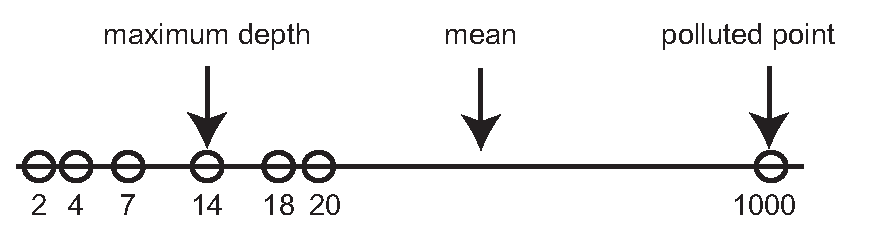
\includegraphics[width=0.8\textwidth]{images/depth_uni.eps}
	\caption{Robustness of halfspace depth for the univariate case}
	\label{fig:hd_uni}	
\end{figure}

Similarly, the halfspace depth of $x$ for the bivariate case is defined by the minimal number of data points in any closed halfspace, which is determined by a hyperplane through $x$ \cite{rousseeuw96RSS}.
In Figure \ref{fig:hd_bi}, the solid line through $x$ is rotated by $180^{\circ}$.
The halfspace depth of $x$ is determined by the smallest portion of data separated by such a hyperplane. For example, the halfspace depth of $x$ is $3/13$, as determined by the dotted line.
However, the halfspace depth of $x$ determined by the solid line is  $4/13$.
\DIFdelbegin \DIFdel{Thus}\DIFdelend \DIFaddbegin \DIFadd{Therefore}\DIFaddend , the halfspace depth of $x$ is $3/13$, which is the minimal number of data points in any closed halfspace through $x$.

\begin{figure}
	\centering
	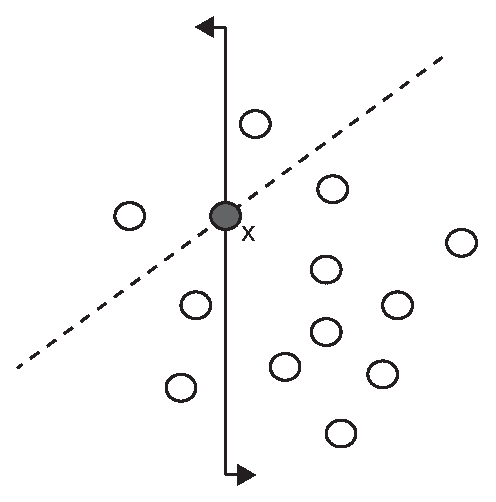
\includegraphics[width=0.6\textwidth]{images/depth_bi.eps}
	\caption{Halfspace depth for the bivariate case}
	\label{fig:hd_bi}	
\end{figure}

The property of halfspace depth is a center-outward ordering of points in $\mathbb{R}^d$ and is affine invariant \cite{Mosler13book}.
These features make halfspace depth \DIFaddbegin \DIFadd{a }\DIFaddend useful tool in nonparametric inference, which leads to various applications such as data classification and cluster analysis \cite{lange14fSP,jeong16acmgis}.
There are multiple approaches to calculating data depth, including halfspace depth \cite{rousseeuw96RSS}, projection depth \cite{wilcox03CSSC}, and simplicial depth \cite{liu90AS}.
While the computational complexity of the projection approach is $\mathcal{O}(n^2)$ (where $n$ is the number of points), the computational complexity of simplicial depth is $\mathcal{O}(n^3)$.
This can significantly increase execution time when $n$ is large.
Thus, this paper uses the more efficient method proposed by \cite{rousseeuw96RSS}, in which the computation complexity for both approaches is $\mathcal{O}(n\log{}n)$.

\subsection{OD Flow Outlier Detection Based on Depth}
The center-outward ordering in data depth is closely related to the detection of outliers.
The upper level sets of data depth in $\mathbb{R}^2$ form the central regions.
The most central region can be regarded as a median.
Conversely, the lower level sets of data depth, which coincide with larger distances from the center, can be regarded as outlyingness.
This concept was utilized by \cite{rousseeuw99AS,aplpackR} to generate bag plots, which are analogous to one-dimensional box plots based on data depth.
This paper uses the bag plot to identify the outliers of OD flows.
Before explaining the method of outlier detection, we first introduce a basic definition of OD flow.

%DIF < \theoremstyle{definition}
%DIF < \begin{definition}{Point.}
%DIF < 	A point $p$ is a tuple $(o,d,t)$, where $o$ and $d$  are the origin and destination ID of  traffic analysis zones and $t$ is the time when the destination ID is recorded.
%DIF < \end{definition}
%DIF < 
%DIF < 
%DIF < \begin{definition}{Trajectory.}
%DIF < 	A trajectory $TR$ is a list of points $(p_1, p_2, p_3,...,p_n)$, where $p_i = (o_i,d_i,t_i)$ and $t_1<t_2<t_3<...<t_n$.
%DIF < \end{definition}
\DIFdelbegin %DIFDELCMD < 

%DIFDELCMD < %%%
\DIFdelend \begin{definition}{Origin-destination (OD) flow.}
	The OD flow $OD_i = (o_i,d_i,c_i,ts_i, te_i)$ is the number of trips from the origin ID to destination ID of traffic analysis zones between the start time ($ts_i$) and the end time ($te_i$), where $ts_i<te_i$.
\end{definition}

Based on this basic \DIFdelbegin \DIFdel{definitions}\DIFdelend \DIFaddbegin \DIFadd{definition}\DIFaddend , Figure \ref{fig:bagplot_0521_0701} depicts bag plots representing the OD flows of New York City taxi data collected on May 21, 2014 and July 1, 2014.
We exploited taxi data on May 21, 2014 because the National September 11 Memorial Museum and Pavilion was opened to the public on this date.
We \DIFaddbegin \DIFadd{also }\DIFaddend randomly selected another data on July 1, 2014.
In Figure \ref{fig:OD_0521}, the deepest depth of OD flows, depth median, is represented by a star symbol.
This point is surrounded by a dark blue bag, which contains the half of OD flows.
This region is regarded as a central region of \DIFaddbegin \DIFadd{the }\DIFaddend OD flows.
The OD flows in the bag are the dominant patterns.
Magnifying the bag by a factor of three, relative to depth median, constructs a fence, as indicated by the light-blue area.
The fence is comparable to the whiskers of a one-dimensional boxplot.
The OD flows outside the fence, represented by red circles, are outliers.
Every OD pair is represented by a point in Figure \ref{fig:bagplot_0521_0701}.
The x-axis indicates the counts of forward OD flows (e.g., the number of OD flows from origin ID $2$ to destination ID $10$), and the y-axis indicates the counts of reverse OD flows (e.g., the number of OD flows from origin ID $10$ to destination  ID $2$) in Figure \ref{fig:OD_0521}.


\begin{figure}
	\centering
	\begin{subfigure}[b]{0.49\textwidth}
		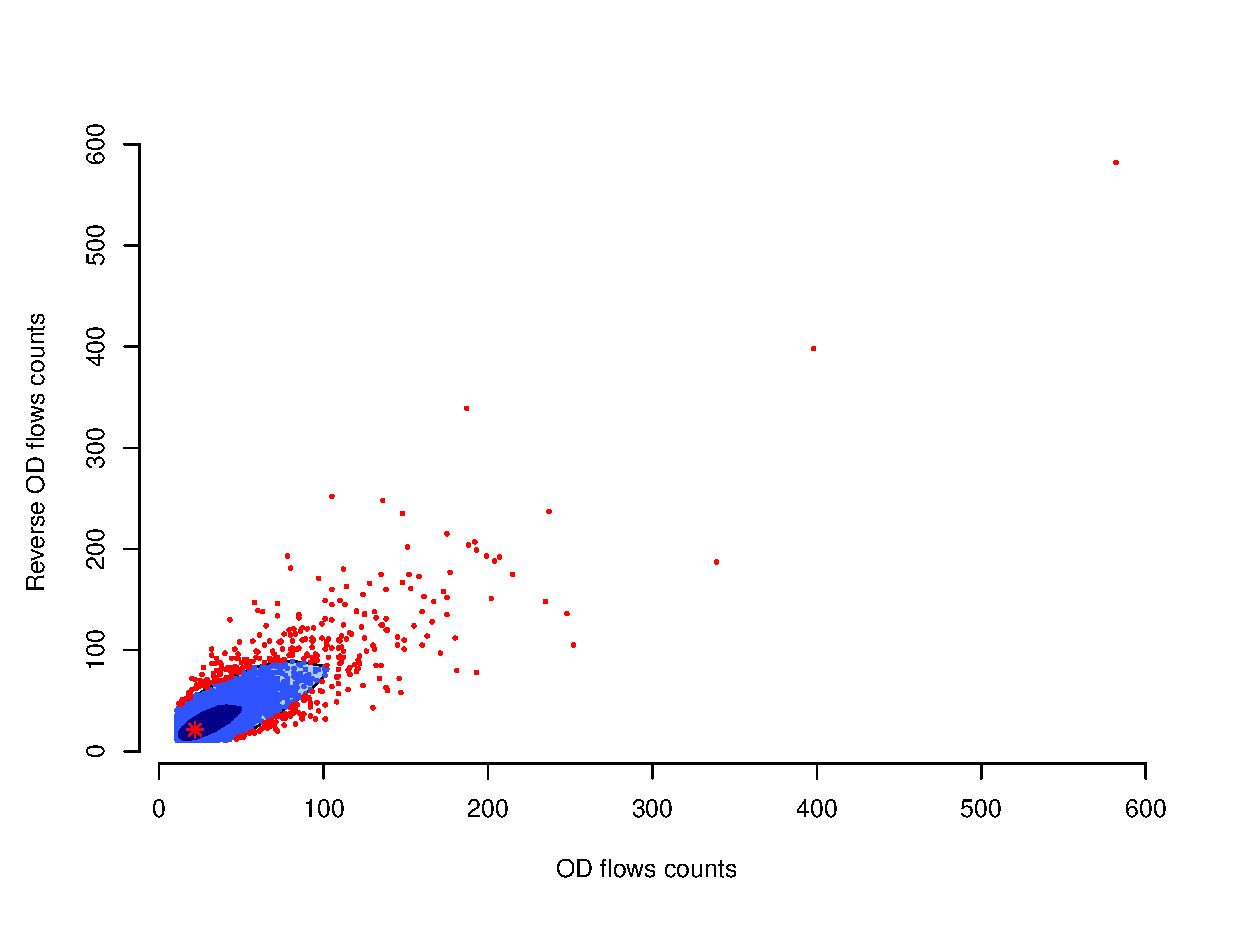
\includegraphics[width=\textwidth]{images/OD_0521.eps}
		\caption{May 21 2014}
		\label{fig:OD_0521}
	\end{subfigure}
	\hfill %add desired spacing between images, e. g. ~, \quad, \qquad, \hfill etc. 	%(or a blank line to force the subfigure onto a new line)
	\begin{subfigure}[b]{0.49\textwidth}
		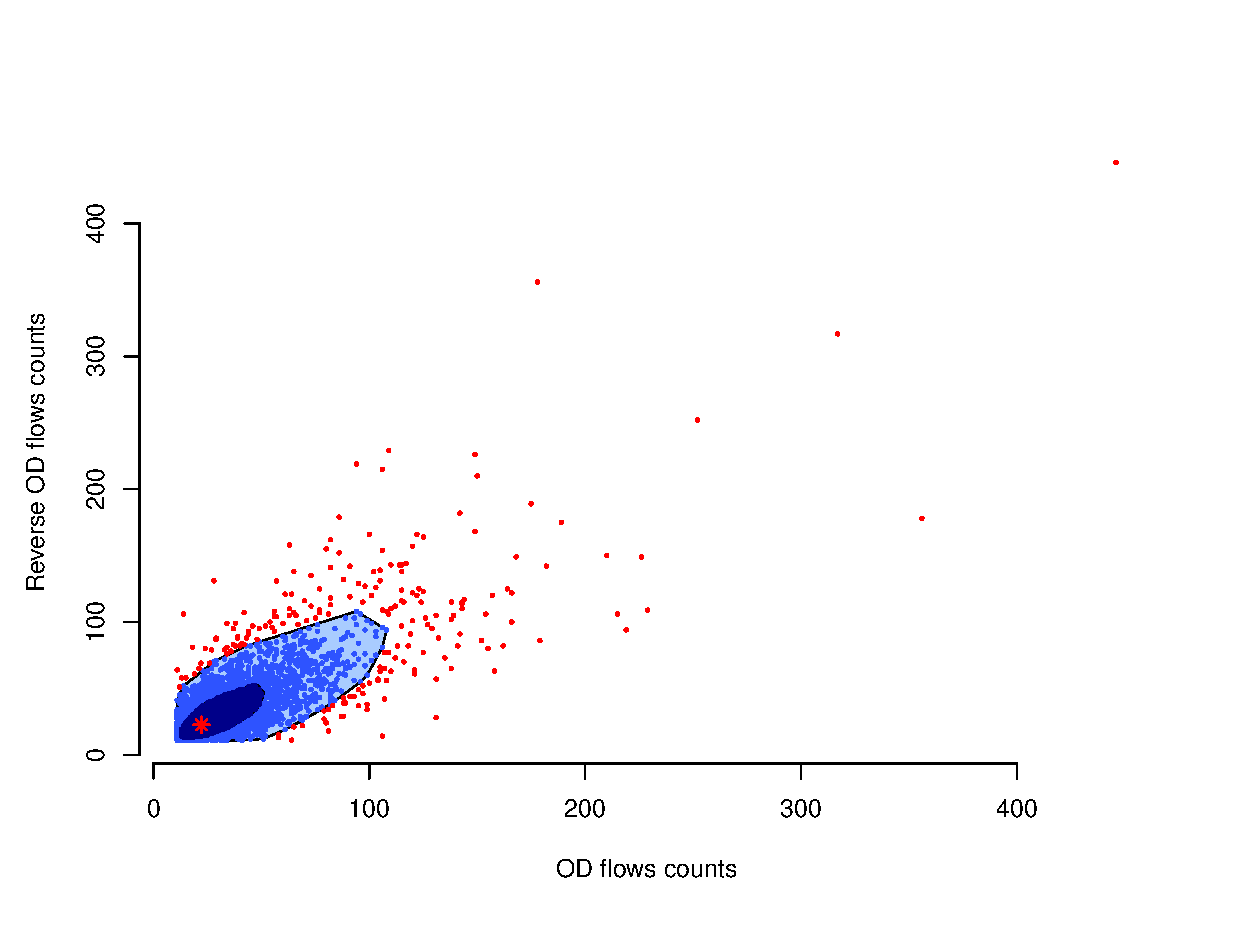
\includegraphics[width=\textwidth]{images/OD_0701.eps}
		\caption{July 1 2014}
		\label{fig:OD_0721}
	\end{subfigure}
    \hfill
	\begin{subfigure}[b]{0.49\textwidth}
	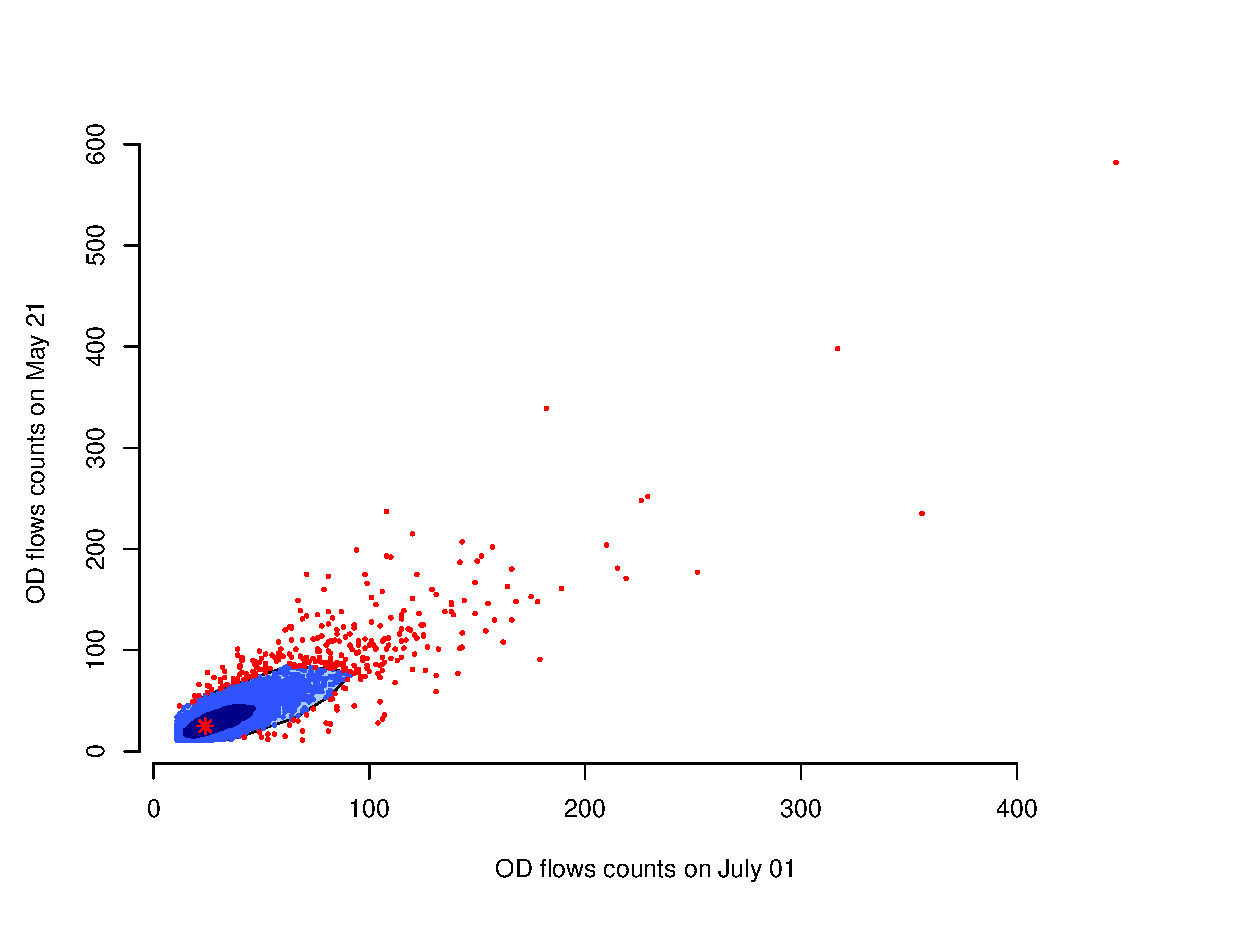
\includegraphics[width=\textwidth]{images/OD_0701_0521.eps}
	\caption{Combination of May 21 and July 1}
	\label{fig:OD_0721_0521}
	\end{subfigure}
    \hfill
	\begin{subfigure}[b]{0.49\textwidth}
	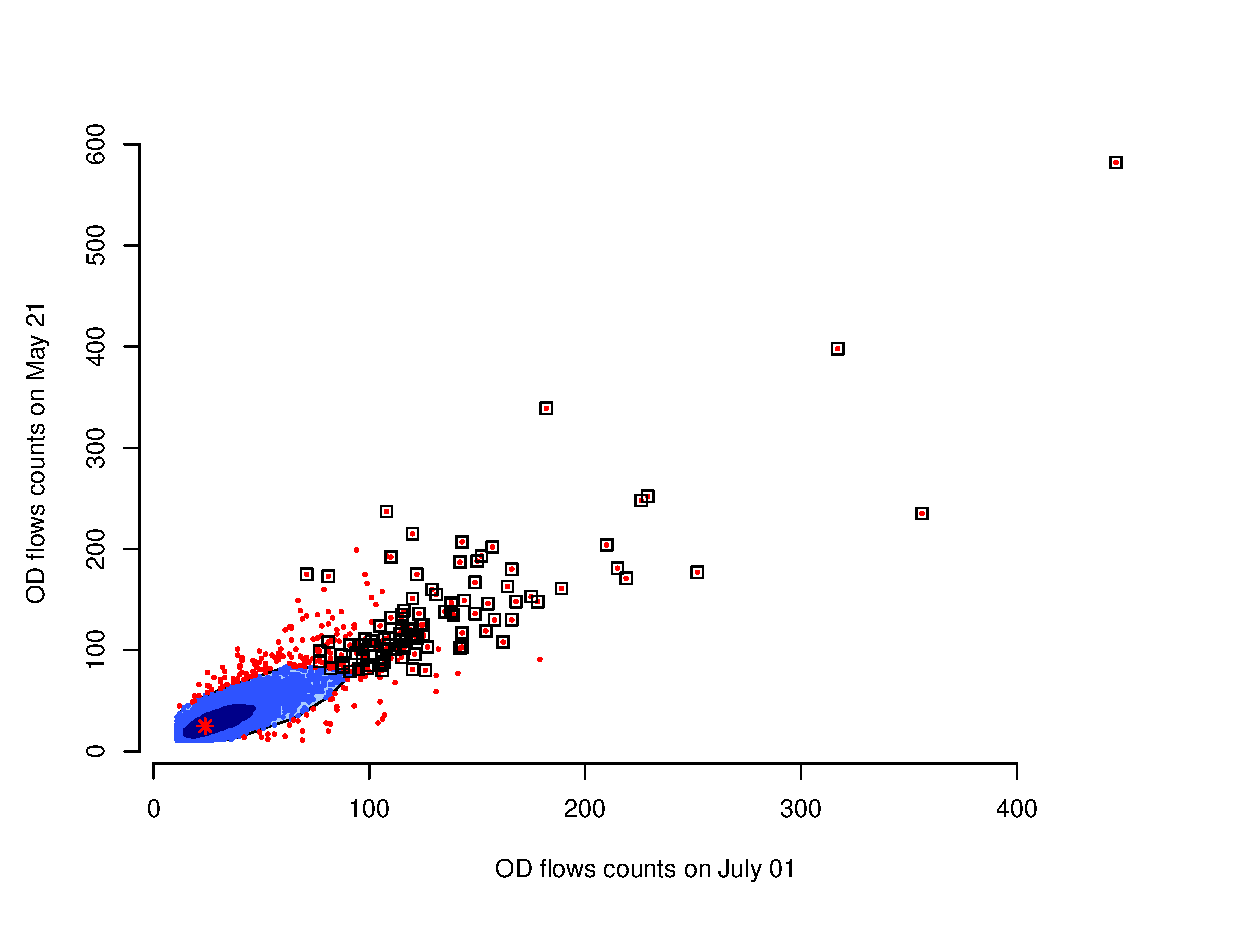
\includegraphics[width=\textwidth]{images/Outliers_high_0701_0521.eps}
	\caption{Detection of outliers with high volume of trips}
	\label{fig:OD_outliers_high}
    \end{subfigure}
	\begin{subfigure}[b]{0.53\textwidth}
	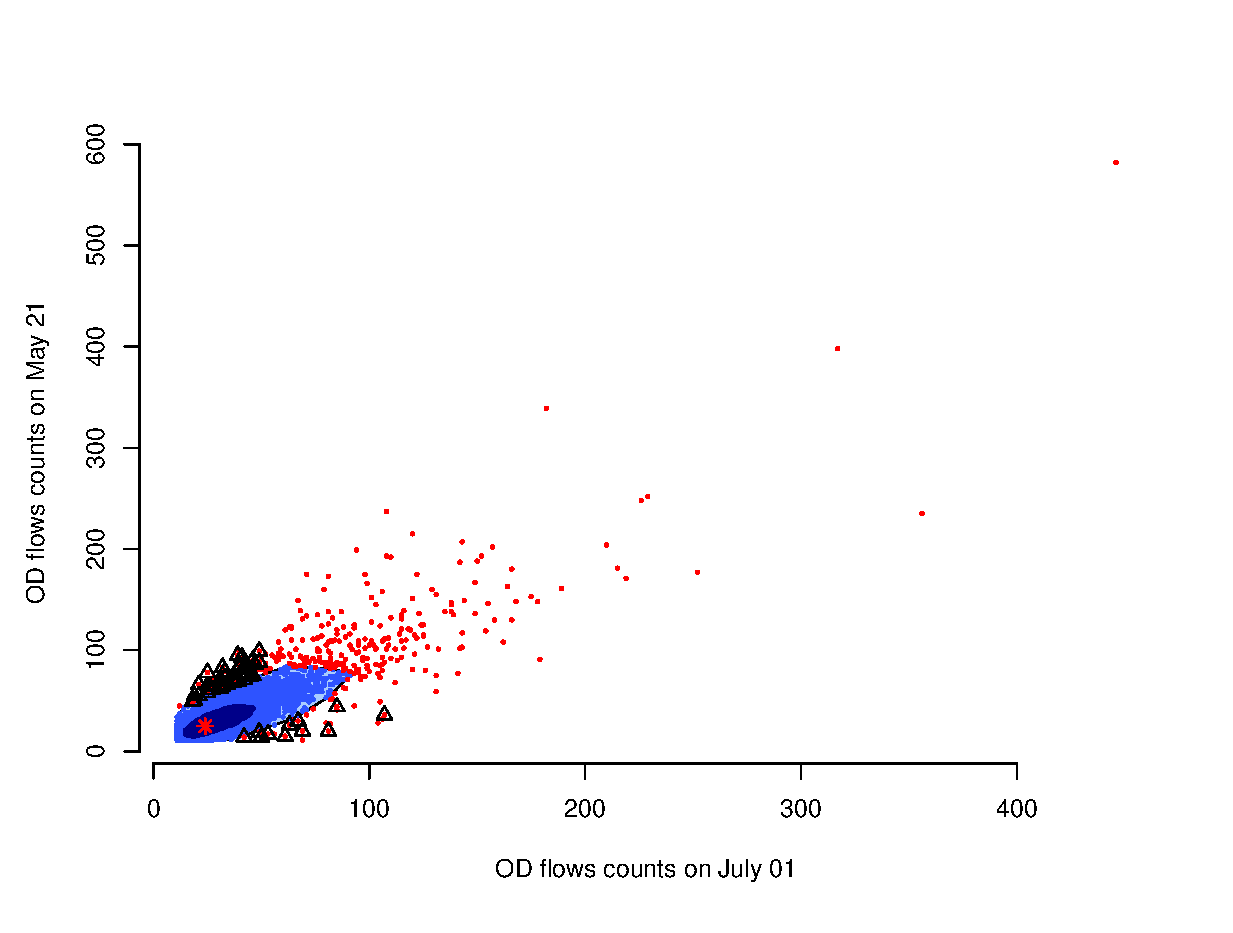
\includegraphics[width=\textwidth]{images/Outliers_rare_0701_0521.eps}
	\caption{Relative outliers detection}
	\label{fig:OD_outliers_rare}
    \end{subfigure}
	\caption{Outliers detection of OD flows using a bag plot}\label{fig:bagplot_0521_0701}	
\end{figure}

The bag plot presents the data using the following attributes: location is represented by the depth median; spread or the spatial extent of bag; correlation or the orientation of the bag; and skewness, as represented by the shape of the bag and the fence \cite{rousseeuw99AS}.
In Figure \ref{fig:OD_0521}, we observe that some forward OD flows have higher counts than their paired reverse OD flows.
We also note the relatively linear correlation between forward OD flows and reverse OD flows and the skewness of forward (reverse) OD flows. 

It is also possible to detect the outliers of OD flows of two different time stamps.
In Figure \ref{fig:OD_0721_0521}, we visualize the OD flows recorded on two \DIFdelbegin \DIFdel{different }\DIFdelend \DIFaddbegin \DIFadd{separated }\DIFaddend days.
Comparing the two sets of OD flows not only indicates the central region of OD flows, it also distinguishes the significantly different OD flows. 

%DIF < Therefore, we can not only see where is the central region of OD flows, but also differentiate which OD flows are significantly different by comparing two sets of different OD flows.
\DIFdelbegin %DIFDELCMD < 

%DIFDELCMD < %%%
\DIFdelend The OD flows in high activity areas of \DIFdelbegin \DIFdel{a }\DIFdelend \DIFaddbegin \DIFadd{the }\DIFaddend city are more likely to have large trip volumes.
We use set operations to detect such outliers.
We regard OD flows on July 1 as the control dataset ($control$); OD flows on May 21 as test dataset ($test$); and the combination of two OD flows as combination dataset ($combination$) in Figure \ref{fig:bagplot_0521_0701}.
Then we can calculate the intersection of three outliers sets ($control \cap test \cap combination$), which are represented as rectangle symbols in Figure \ref{fig:OD_outliers_high}. 

In addition, it is interesting to detect the outliers of OD flows which are typical patterns at time $t_1$ \DIFdelbegin \DIFdel{and atypical behavior }\DIFdelend \DIFaddbegin \DIFadd{but atypical behaviors }\DIFaddend at time $t_2$.
We define the union of points in the bag, the central region, at time $t_1$ and $t_2$.
Then we calculate the intersection of two sets\DIFdelbegin \DIFdel{, }\DIFdelend \DIFaddbegin \DIFadd{: }\DIFaddend the outliers of the combination set and the previous union set.
These outliers are represented as triangle symbols in Figure \ref{fig:OD_outliers_rare}.
These outliers are typical OD flows at time $t_1$, located in the central regions in the bag plot.
When we consider two OD flows together, they become unusual OD flows, some have more trips and some have less trips, relative to the control dataset.
Thus, we can detect and treat outliers interactively based on data depth.

%DIF <  we regard OD flows on July 01 ($t_1$) as control data set($control$) and OD flows on May 21 ($t_2$) as test data set ($test$). From the combination of two OD flows set ($combination$, see Figure \ref{fig:OD_0721_0521}), we calculate the interaction of the combination of two OD flows set and the test data set ($B = \{combination \cap test\}$). We also calculate the difference between the combination of two OD flows set and the control data set ($A = \{combination - control\}$) . Finally, we can detect the outliers of OD flows based on the difference between two sets $A$ and  $B$ ($C = \{A - B\}$). The triangles indicate these outliers in Figure \ref{fig:OD_outliers}.
\DIFdelbegin %DIFDELCMD < 

%DIFDELCMD < %%%
\DIFdelend \subsection{OD Flow Comparisons Based on Depth}
Data depth can compare bivariate data from two independent groups.
A t-test can be used to compare means from two independent groups.
For example, the t-test reveals whether the means of two OD flows are different at two different temporal ranges.
However, it is also worth examining how groups differ in terms of scale, which is also referred to as spread.
Comparisons of central regions in data depth evaluate the marginal distribution, thereby considering the overall structure of the data \cite{wilcox03MBR}.

Let $X$ and $Y$ be the random variables having distributions F and G for two independent groups.
The quality index proposed by \cite{liu93JASA} is the probability that the depth of $Y$ is greater than or equal to depth of $X$. 

\begin{equation*}
Q(F,G) = P[D(X;F) \leq D(Y;F)],
\end{equation*}

where $P$ is the probability and $D(X;F)$ is the depth of randomly sampled observations according from distribution $F$.
The range of $Q$, as presented by \cite{liu93JASA}, is $[0,1]$ and $Q(F,G) = 0.5$ if and only if $F = G$. If $Q < 0.5$  or if $Q > 0.5$, the scale increases or decreases from  $F$ to $G$.
Therefore, it is possible to detect differences in scale using a bootstrap method.

Let $X_1,...,X_a$ be a random sample from $F$, and $Y_1,...,Y_b$ be a random sample from $G$.
The estimate of $Q(F,G)$ is calculated as shown below.

\begin{equation*}
\hat{Q}(F,G) =\frac{1}{b} \sum_{i=1}^{b} R(Y_i;F_a),
\end{equation*}

where $R(Y_i;F_a)$ indicates the proportion of $X_j$ which has $D(X_j;F_a) \leq D(Y_i;F_a)$.
Similarly, the estimate of $Q(G,F)$ can be defined as follows:

\begin{equation*}
\hat{Q}(G,F) =\frac{1}{a} \sum_{i=1}^{a} R(X_i;G_b).
\end{equation*}

Bootstrap samples are obtained by resampling from the two groups ($F$ and $G$).
Under the null hypothesis ($H_0: Q(F,G) = Q(G,F)$), the difference of the resulting bootstrap estimates is $Q^*(F,G) - Q^*(G,F)$.
\DIFdelbegin \DIFdel{Thus}\DIFdelend \DIFaddbegin \DIFadd{Therefore}\DIFaddend , if the confidence interval of $Q(F,G) - Q(G,F)$ does not contain zero, we can reject the null hypothesis, $H_0$ \cite{liu93JASA,wilcox03MBR}.

\begin{figure}
	\centering
	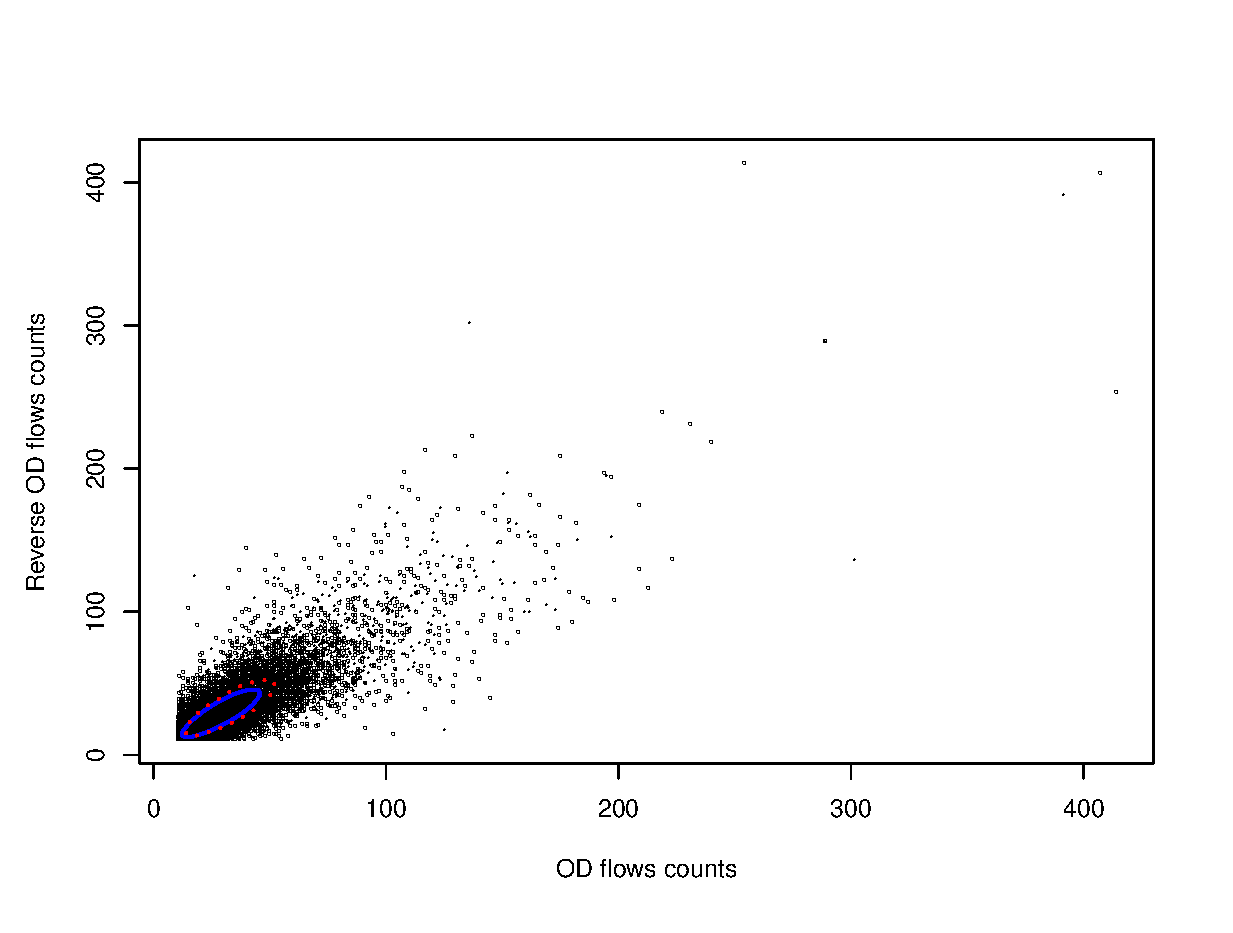
\includegraphics[width=0.6\textwidth]{images/com_mar_0329.eps}
	\caption{Central regions of two OD flows: $\circ$ indicates the OD flows for Saturday, March 29 2014 and * indicates the OD flows for a list of Saturdays; blue line presents the central region of the OD flows for the list of Saturdays and red dotted line presents the central region of the OD flows on March 29.}
	\label{fig:com_mar_0329}	
\end{figure}

For \DIFaddbegin \DIFadd{the }\DIFaddend ease of understanding, Figure \ref{fig:com_mar_0329} presents the central regions of two OD flows.
One dataset is OD flows for Saturday, March 29, 2014, and the other dataset includes multiple Saturdays, those of March 1, 8, 15, 22, and April 5.
At 552,064 taxi trips, the day of March 29 had the highest number of taxi trips for the year of 2014.
The dataset for the other five Saturdays comprised 2,621,703 taxi trips.
The bootstrap method reveals that the confidence interval is 0.0247 and 0.0596.
This confidence interval does not include zero, thus rejecting the $H_0$ null hypothesis.
This indicates that the amount of scale is significantly changed between two OD flow datasets.
Furthermore, the OD flows from the group of Saturdays \DIFdelbegin \DIFdel{is }\DIFdelend \DIFaddbegin \DIFadd{are }\DIFaddend nested within the OD flows corresponding to March 29. This additional perspective \DIFdelbegin \DIFdel{was }\DIFdelend \DIFaddbegin \DIFadd{is }\DIFaddend based on data depth comparisons. 

The bootstrap method is a time consuming process.
For this study, we generate $2,000$ bootstrap samples.
To improve the execution efficiency of the bootstrap computation, we distributed the work across multiple \DIFaddbegin \DIFadd{computing }\DIFaddend nodes and cores by implementing an embarrassingly parallel R code. 
%DIF <  Thus, we can effectively improve  execution efficiency.
%DIF <  investigate resource pressures between serial and parallel approaches in the following section.


\section{Experiments}
\label{sec:experiments}

\subsection{Data}
This study uses New York City taxi data collected in 2014 to evaluate the effectiveness of the proposed approach.
Figure \ref{fig:taxizone} presents traffic analysis zones in New York City which indicate the origin and the destination IDs of the OD flows. 
A traffic analysis zone (TAZ) is the most commonly adopted basic geographic unit in transportation planning models.
The geographic areas of TAZ are delineated by transportation officials for tabulating traffic-related data.
The size of TAZ varies because it accounts the underlying population in each zone, which consists of one or more census blocks, block groups, or census tracts.
The shapes of the TAZs in this study are derived from the cartographic boundary shapefiles developed by the U.S. Census Bureau in conjunction with the 2010 census (https://www2.census.gov/geo/tiger/TIGER2010/TAZ/2010/).
Considering the TAZs are particularly useful for journey-to-work and place-of-work statistics, we employed them as the basic units for accounting the taxi trips. 
Figure \ref{fig:ODflows} shows OD flows on July 1.
Red lines indicate the dominant OD flows.

\begin{figure}
	\centering
	\begin{subfigure}[b]{0.49\textwidth}
		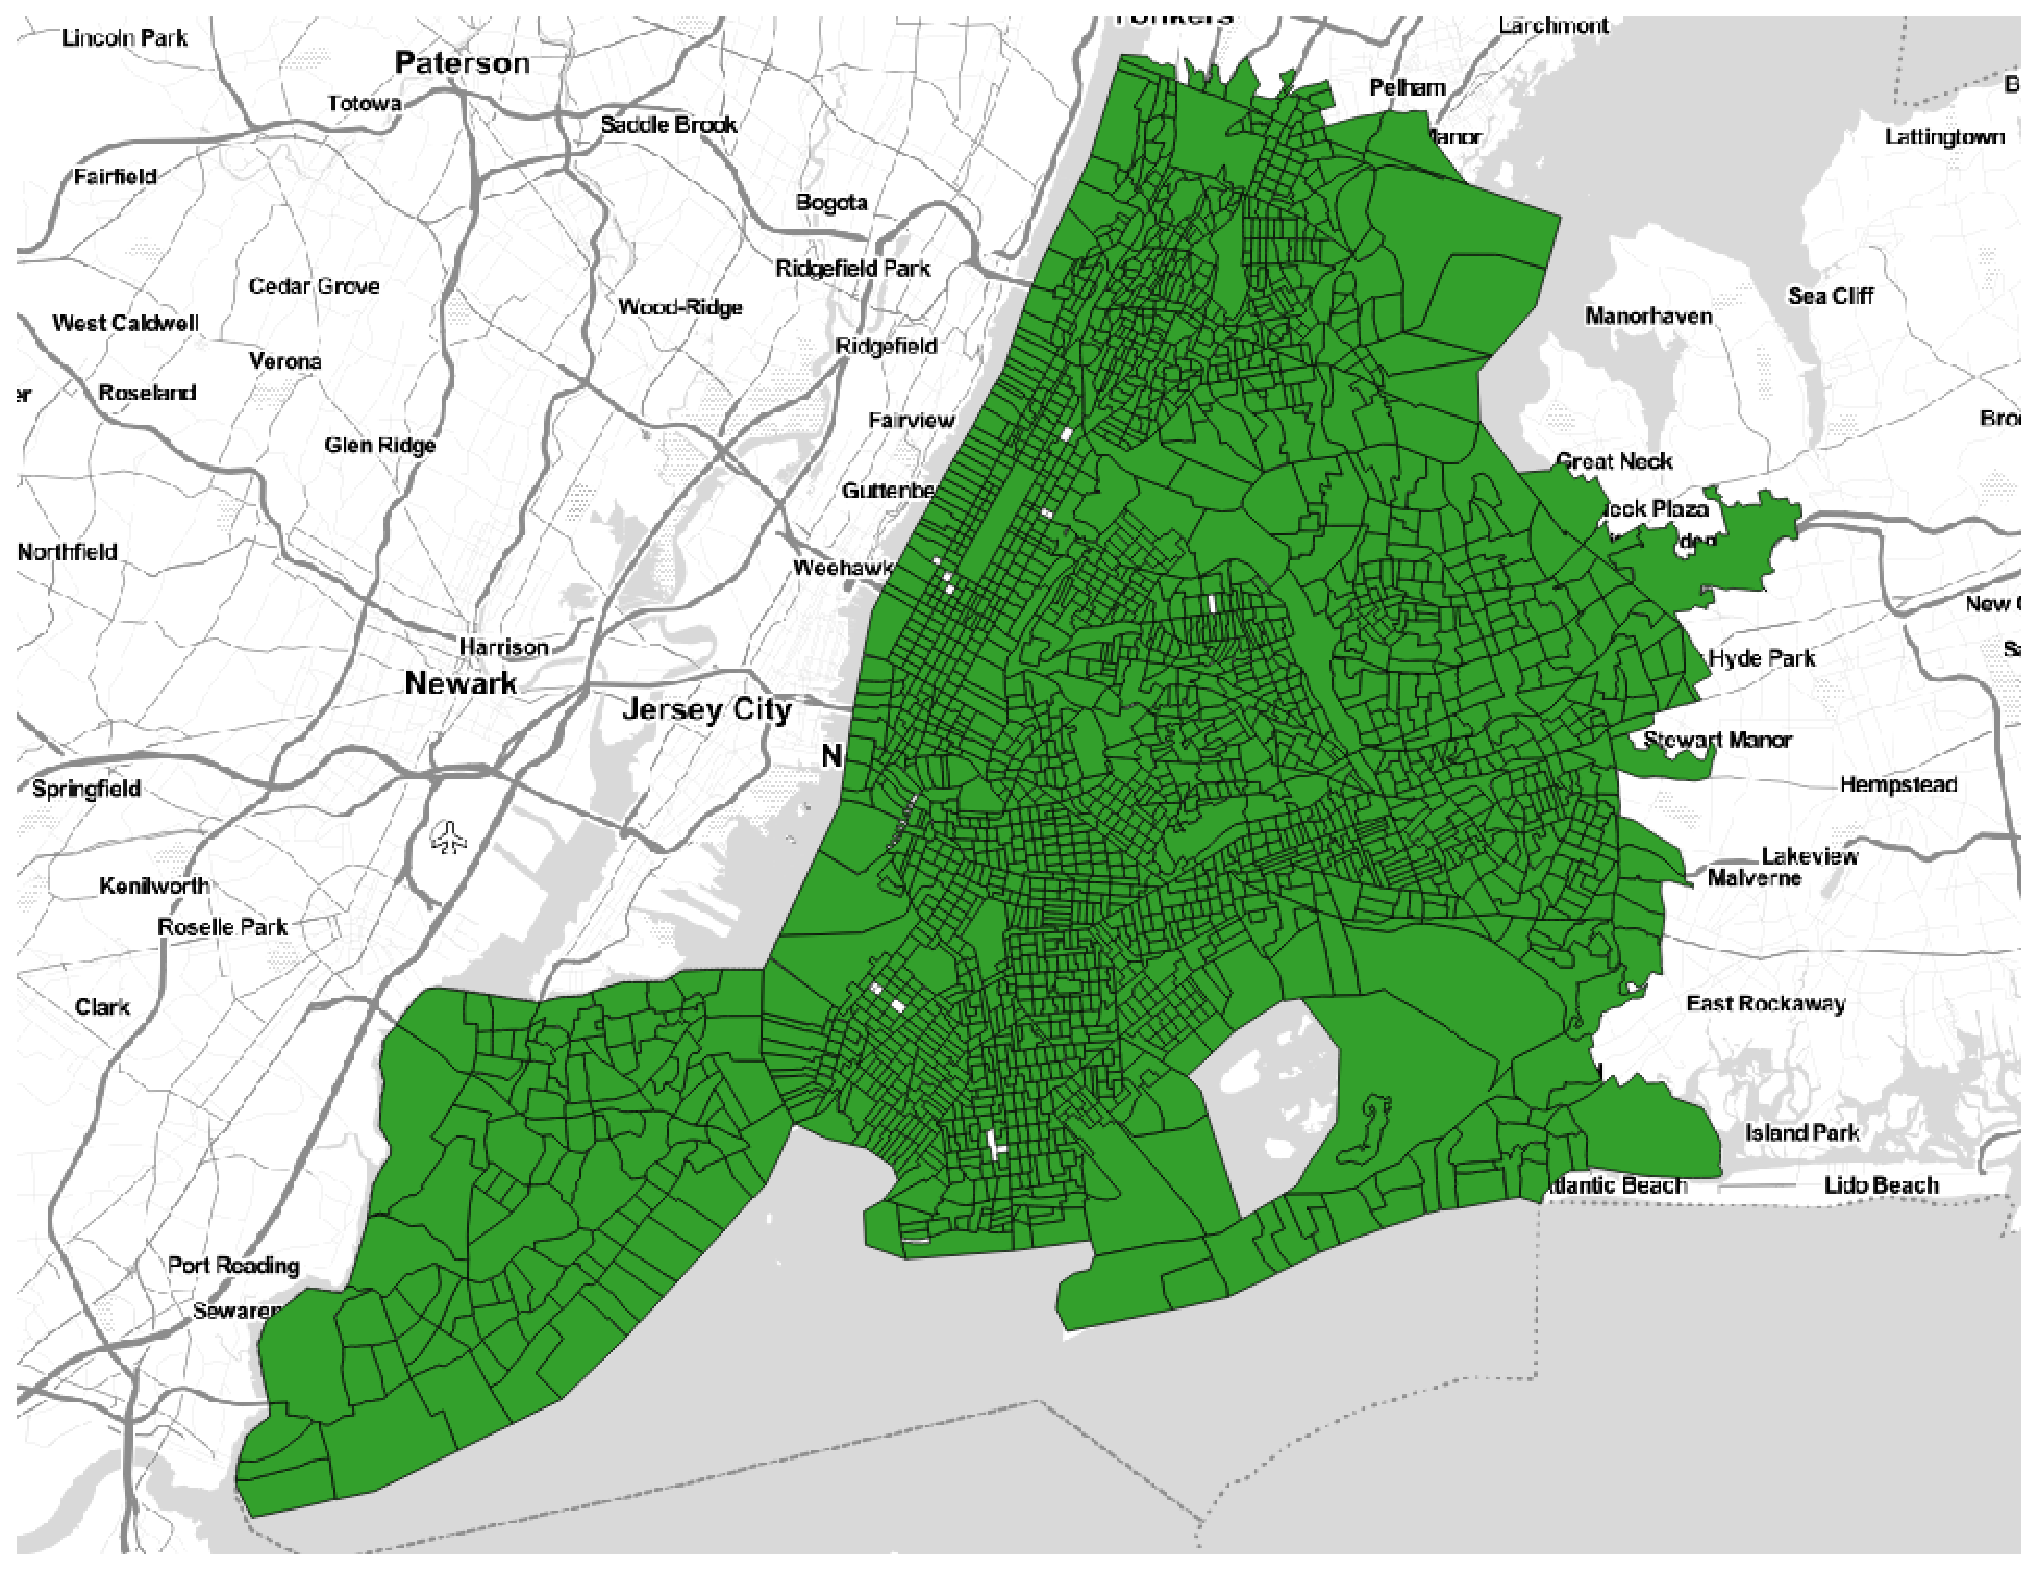
\includegraphics[width=\textwidth]{images/taxizone.eps}
		\caption{2,250 traffic analysis zones in New York City}
		\label{fig:taxizone}
	\end{subfigure}
	\hfill
	%DIF < add desired spacing between images, e. g. ~, \quad, \qquad, \hfill etc. 	%(or a blank line to force the subfigure onto a new line)
	\begin{subfigure}[b]{0.49\textwidth}
		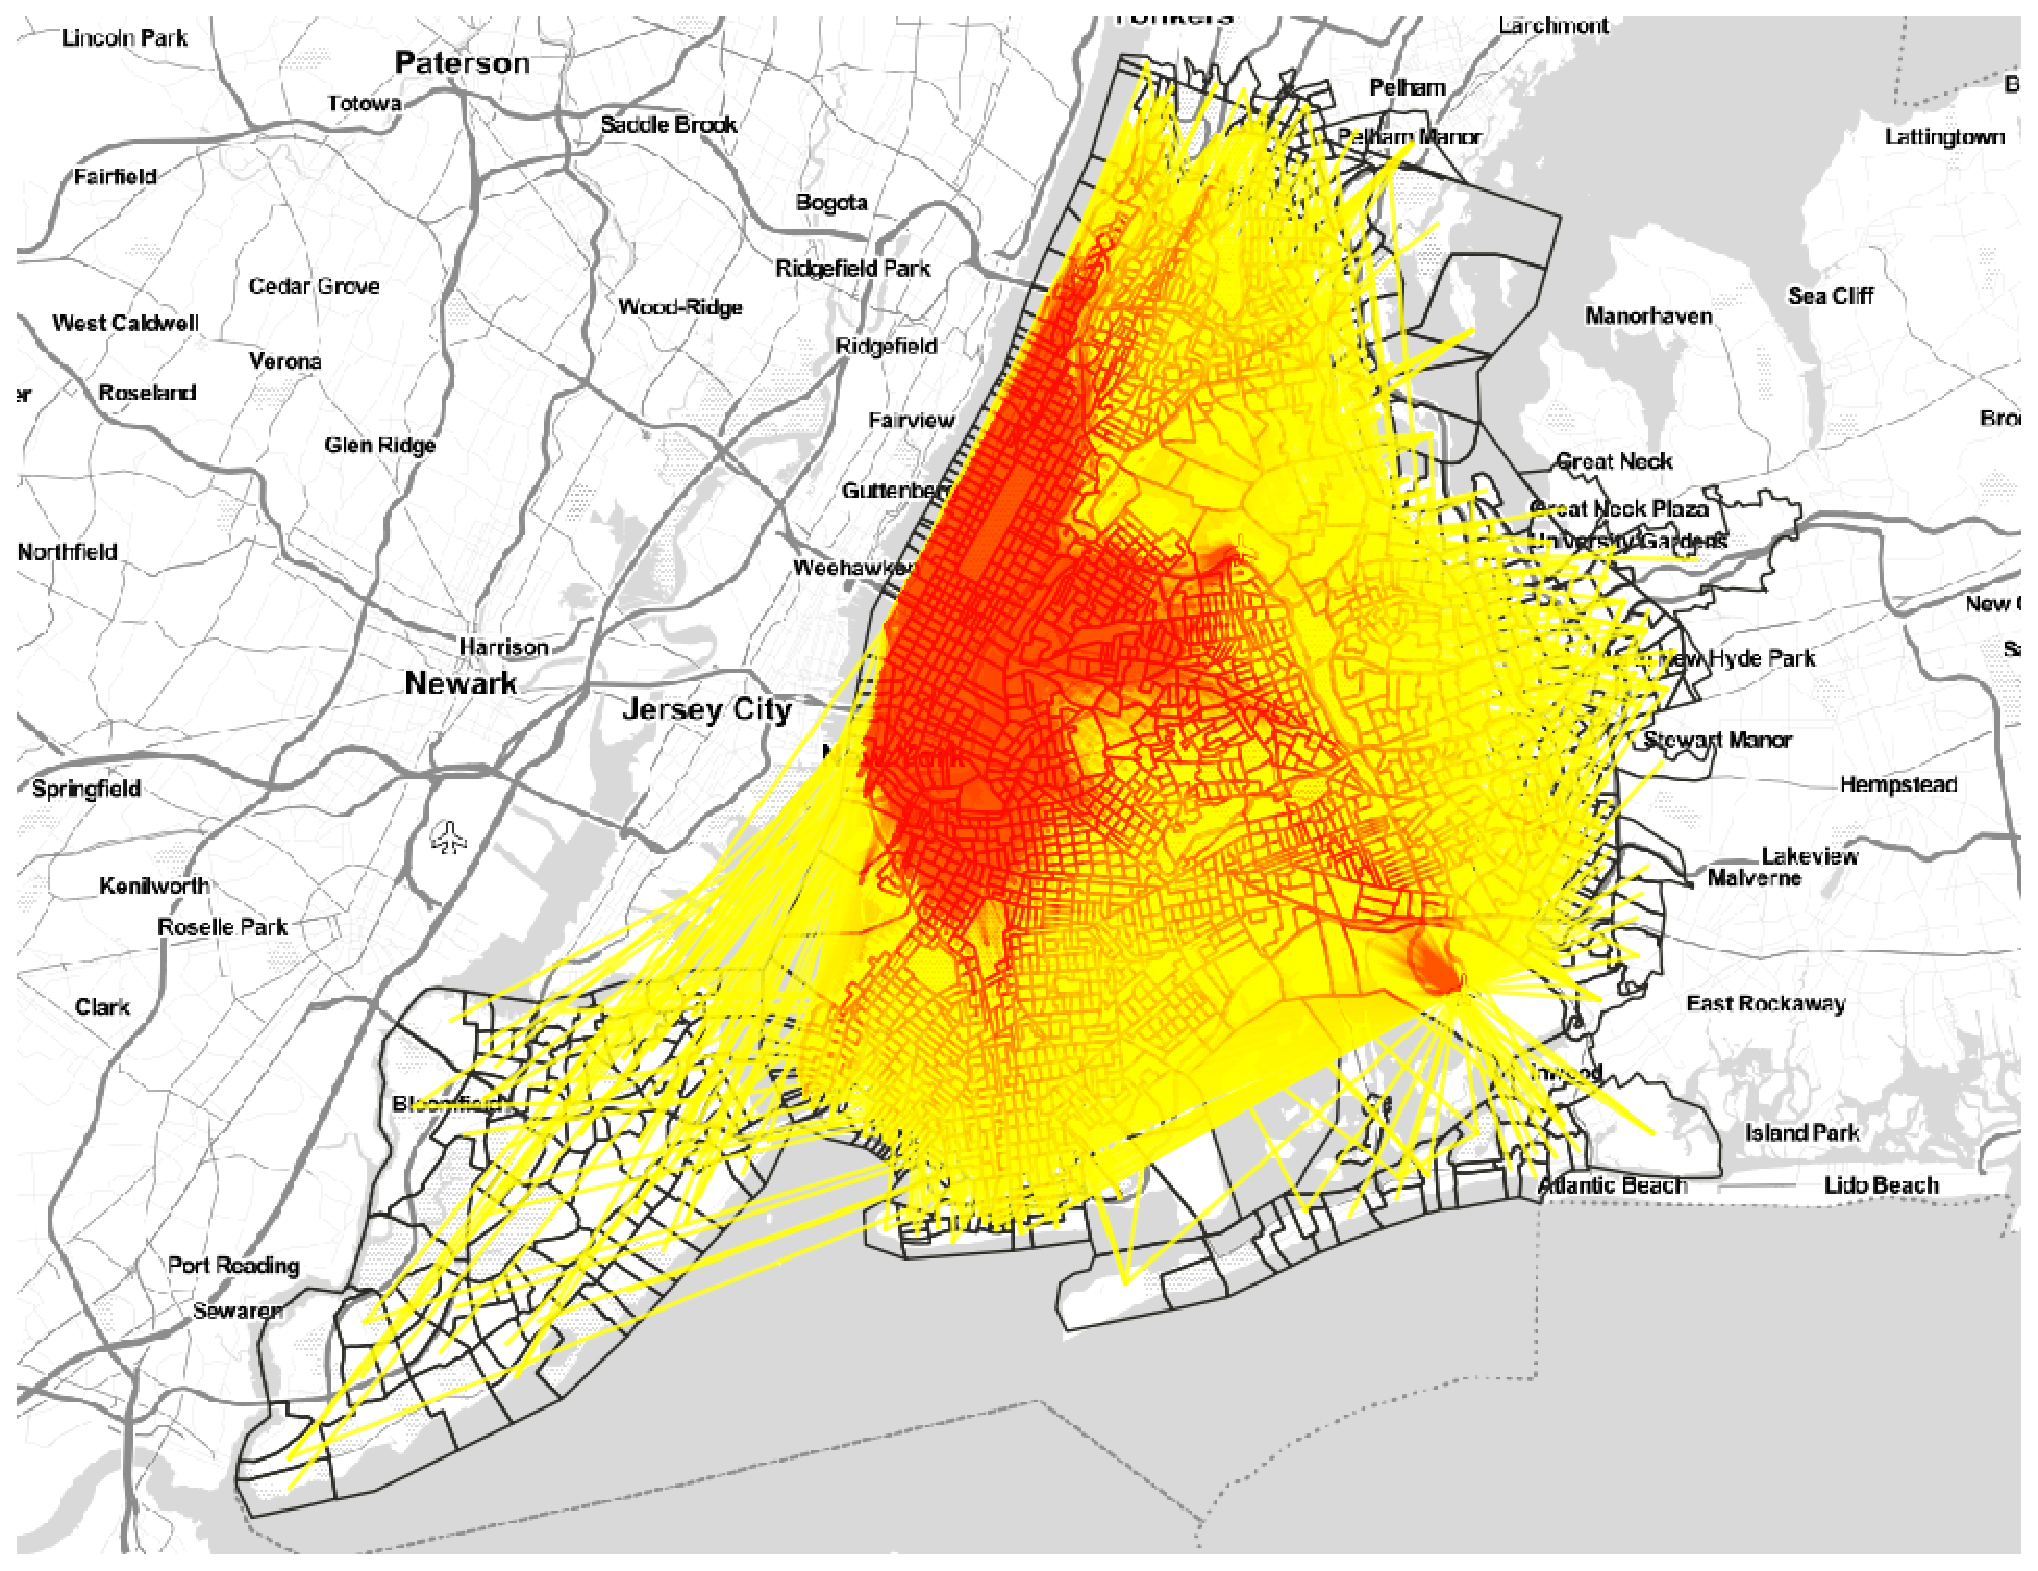
\includegraphics[width=\textwidth]{images/July1st_pic2.eps}
		\caption{OD flows on July 1 2014}
		\label{fig:ODflows}
	\end{subfigure}
	\caption{Experimental data: New York City taxi data}\label{fig:taxi_data}	
\end{figure}

As a case study, this paper examined OD flows recorded on weekdays and weekends in June 2014.
The weekday dataset includes taxi trajectories collected on June 3, 10, 17, and 24, and represents 1,721,655 taxi trips.
The weekend dataset includes taxi trajectories collected on June 8, 15, 22, and 29, and describes 1,593,480. 

\subsection{Procedure}

The performance of the proposed method was compared with alternative methods.
Trajectory anomaly detection based on Mahalanobis distance \cite{pan13ACMGIS} was used to evaluate the performance of outlier detection by the proposed method.
The Mahalanobis distance is distinguished from Euclidean distance by its consideration of the correlations of the data, in this case, the two OD flow datasets. 
According to \cite{pan13ACMGIS}, the anomaly detection threshold can be defined as follows:

\begin{equation*}
d_M(OD_{t_1}, \mu_{[t_0,t_1)}) \geq 3\cdot \sqrt{\frac{1}{N}\sum_{t \in [t_0,t_1)} (OD_{t} - \mu_{[t_0,t_1)})^2} .
\end{equation*}

where $OD_{t_1}$ is the current OD flow, and $\mu_{[t_0,t_1)}$ is the median of all OD flows during $[t_0,t_1)$.
In addition, we visualized the results in order to compare them and make the difference easier to understand.
The difference of scale was evaluated using standard statistics, such as F-test, to compare the variance of two datasets. 

For data cleaning process, this study used Hadoop with Pig.
We developed a Hadoop program to handle the large \DIFdelbegin \DIFdel{volume of data }\DIFdelend \DIFaddbegin \DIFadd{data volume}\DIFaddend , which was composed of 173 million taxi trip records, remove trips with invalid OD coordinates, and assign each OD locations into the corresponding traffic analysis zone.
To implement the OD flow outlier detection, this study used R.
The computing environment used Amazon Web Service and the Bridges supercomputer at the Pittsburgh Supercomputing Center. 
This study only evaluated OD flows more than 10 trips, as the low trip number OD flows could have distorted the view of the data.
All the code will be released as open source (the link to the code \DIFdelbegin \DIFdel{will added later and currently }\DIFdelend is available upon request).


%DIF < Further, we used OD flows that have more than 10 trips. It is reasonable to remove the majority of low number of OD flows, which may distort the view of the data. All the code will be released as open source (the link to the code will added later and currently is available upon request).
\DIFdelbegin %DIFDELCMD < 

%DIFDELCMD < %%%
%DIF < With regard to data cleaning process, this study used Hadoop with Pig. R was used to implement the code in Amazon Web Service  and Bridges supercomputer resources. Further, we used OD flows that have more than 10 trips. It is reasonable to remove the majority of low number of OD flows, which may distort the view of the data. 
%DIFDELCMD < 

%DIFDELCMD < %%%
%DIF < Data cleaning process
%DIFDELCMD < 

%DIFDELCMD < %%%
\DIFdelend \subsection{Case study: weekdays vs weekends}
\subsubsection{Outlier Detection}
The bag plots presented OD flow outliers on weekdays and weekends in Figures \ref{fig:weekdays_bag} and \ref{fig:weekends_bag}, respectively.
The outliers are detected by considering forward OD flows and reverse OD flows together.

\begin{figure}
	\centering
	\begin{subfigure}[b]{0.49\textwidth}
		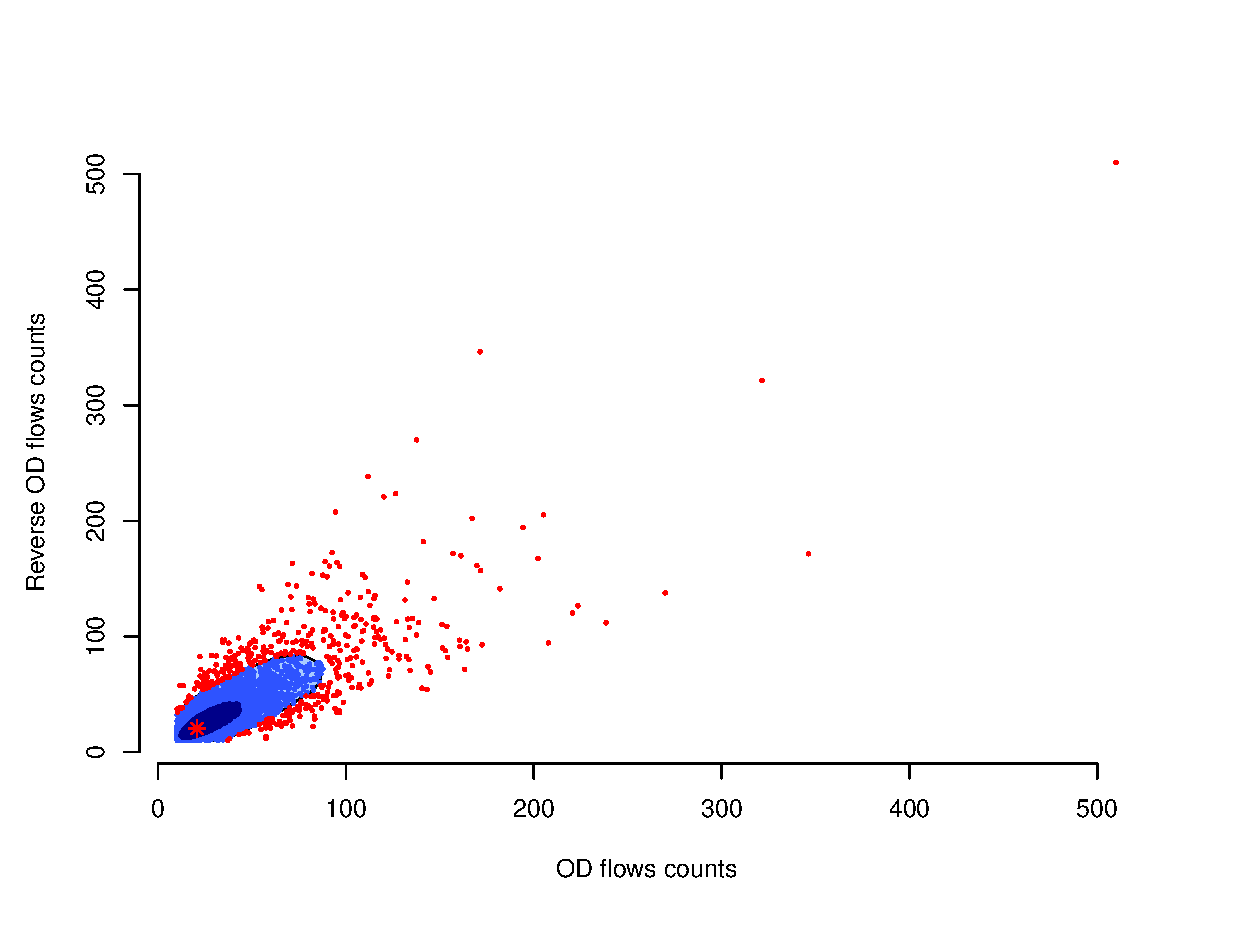
\includegraphics[width=\textwidth]{images/OD_weekdays.eps}
		\caption{Bag plot on weekdays}
		\label{fig:weekdays_bag}
	\end{subfigure}
	\hfill %add desired spacing between images, e. g. ~, \quad, \qquad, \hfill etc. 	%(or a blank line to force the subfigure onto a new line)
	\begin{subfigure}[b]{0.49\textwidth}
		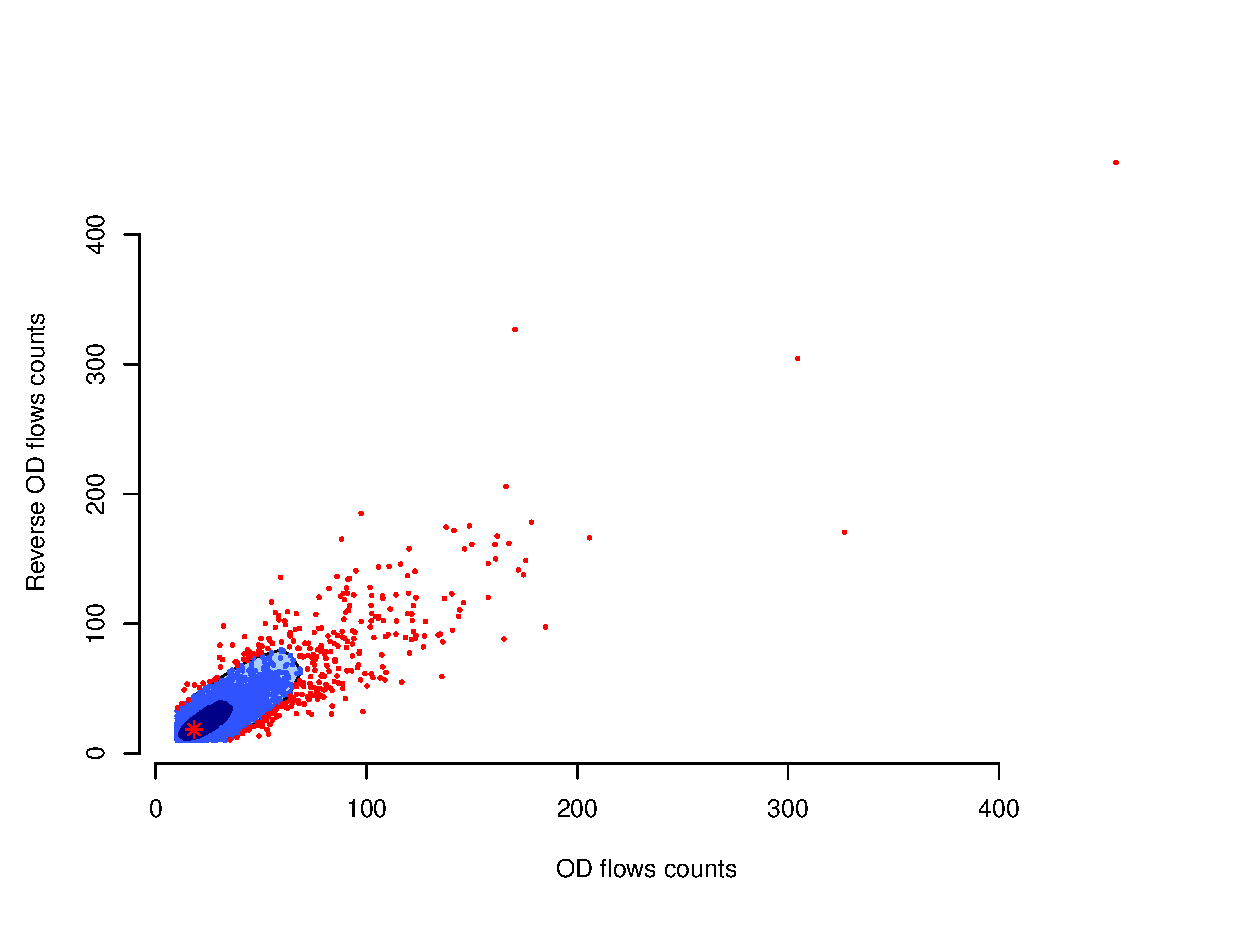
\includegraphics[width=\textwidth]{images/OD_weekends.eps}
		\caption{Bag plot on weekends}
		\label{fig:weekends_bag}
	\end{subfigure}
	\caption{Outliers detection of OD flows: X-axis indicates forward OD flows counts and Y-axis indicates reverse OD flows counts.}\label{fig:week_weekends_bag}	
\end{figure}

To find the difference between two datasets, we considered two forward OD flows together with the bag plot.
Then, we identified the outliers OD flows in Figure \ref{fig:weekdays_high}.
The outliers with rectangle symbols indicate OD flows with large volumes of taxi trips during weekdays and weekends.
Figure \ref{fig:weekdays_high_map} depicts these outliers are superimposed on a map with red lines.
The yellow lines represent the other OD flows, excluding the large volume OD flows on weekdays and weekends. 

This case clearly demonstrates that most OD flows occurred in three broad areas: within Manhattan, between the center of Manhattan and the two major airports (J.F.K International Airport and LaGuardia Airport), and between the two airports.


\begin{figure}
	\centering
	\begin{subfigure}[b]{0.49\textwidth}
		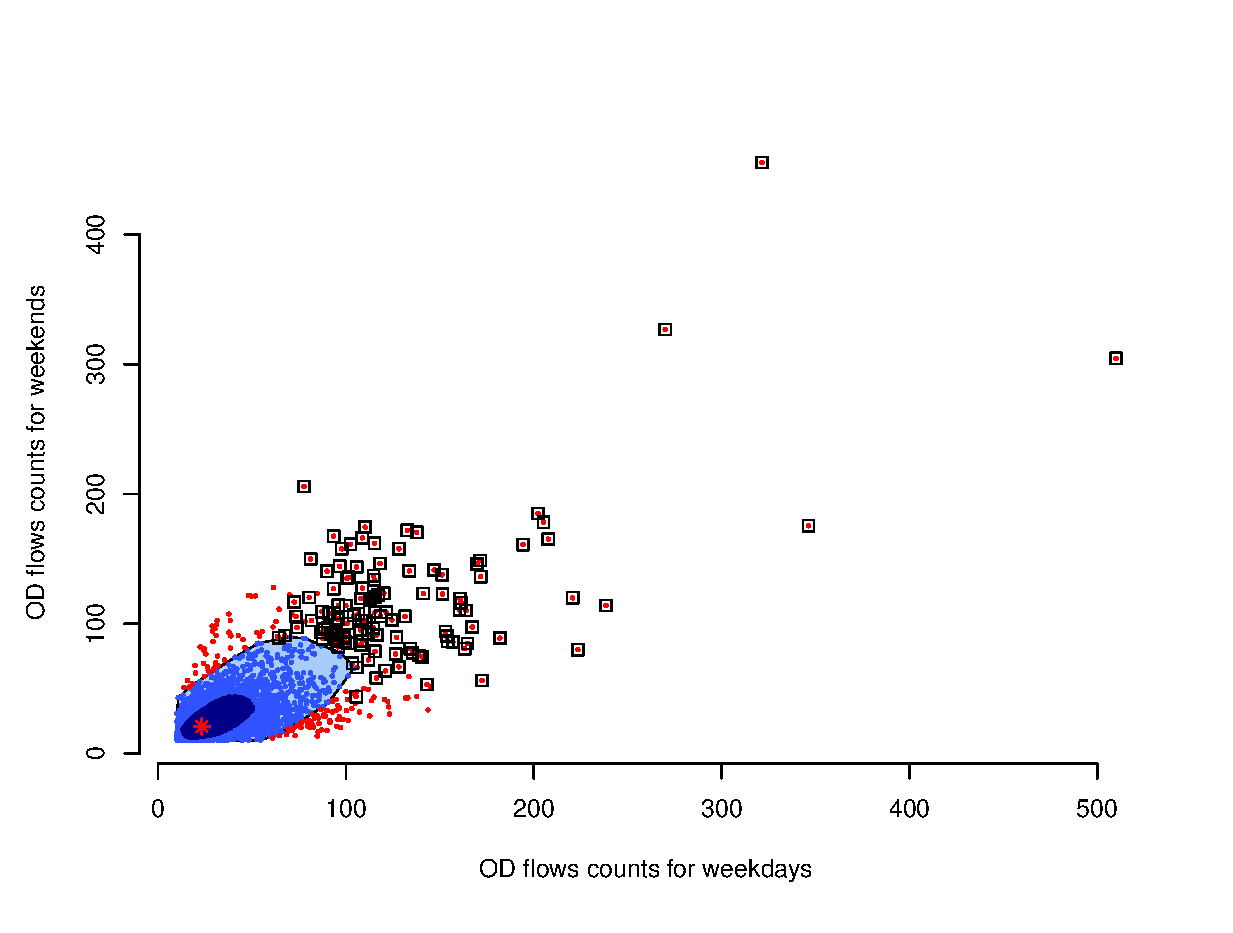
\includegraphics[width=\textwidth]{images/Outliers_high_weekdays_weekends.eps}
		\caption{OD flows with high volume of trips}
		\label{fig:weekdays_high}
	\end{subfigure}
	\hfill %add desired spacing between images, e. g. ~, \quad, \qquad, \hfill etc. 	%(or a blank line to force the subfigure onto a new line)
	\begin{subfigure}[b]{0.49\textwidth}
		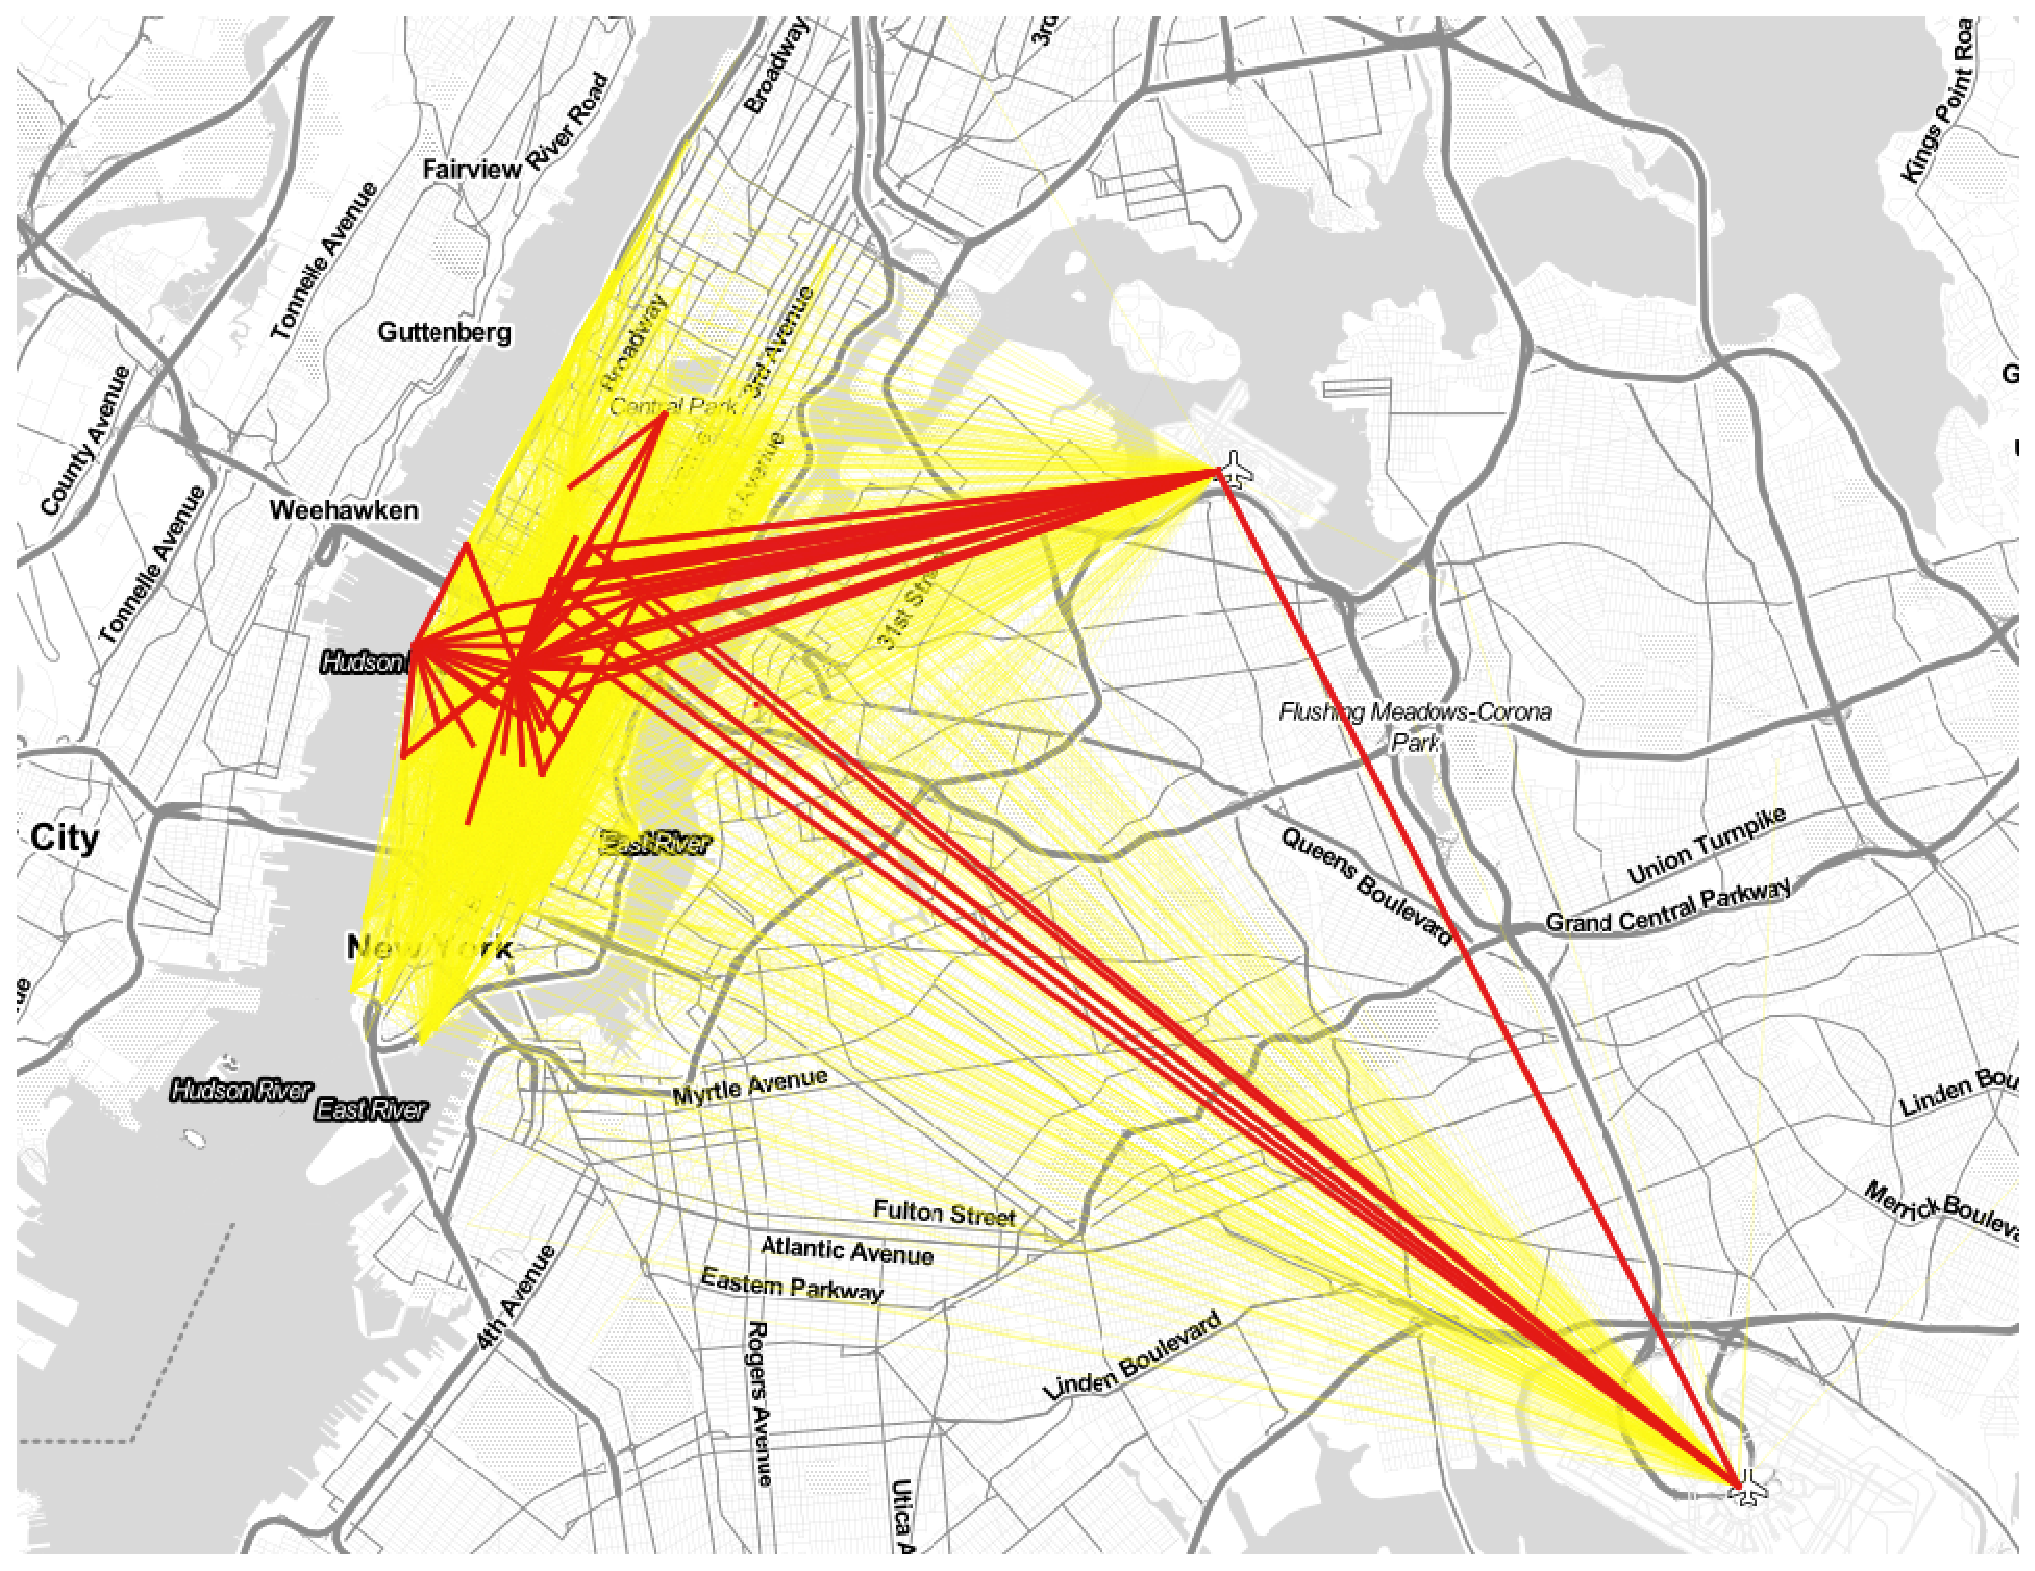
\includegraphics[width=\textwidth]{images/outliers2_high_weekdays_weekends.eps}
		\caption{OD flow map with high volume of trips}
		\label{fig:weekdays_high_map}
	\end{subfigure}
	\caption{Outliers with high volume of trips on weekdays and weekends: Rectangles in Figure \ref{fig:weekdays_high} coincide with red lines in Figure \ref{fig:weekdays_high_map}. }\label{fig:weekdays_high_OD_map}	
\end{figure}

In addition, we investigated abnormal weekend OD flows that are typical weekday OD flows.
These abnormal weekend OD flows exhibited substantial variance in number of taxi trips relative to their weekday counterparts.
Figure \ref{fig:weekdays_rare} presents these OD flows outliers with triangle symbols.
In Figure \ref{fig:weekdays_rare_map}, red lines indicate the substantial increases in weekend trip volumes.
Conversely, blue lines indicate the decreases in trip volume.
Figure \ref{fig:weekdays_rare_map} reveals that OD flows between the center of Manhattan and the two airports or between the two airports were not significantly different during weekdays and weekends. 
However, we did observe some meaningful decrease in OD flows during the weekends in business district, as depicted by the blue lines in Figure \ref{fig:weekdays_rare_map}.


%DIF <   decreased significantly during weekdays and weekends (e.g., left-side blue OD flows in business district in Figure \ref{fig:weekdays_rare_map}).
\DIFdelbegin %DIFDELCMD < 

%DIFDELCMD < %%%
%DIF < These OD flows are represented on a map with red lines in Figure \ref{fig:weekdays_rare_map}.
%DIFDELCMD < 

%DIFDELCMD < %%%
\DIFdelend \begin{figure}
	\centering
	\begin{subfigure}[b]{0.49\textwidth}
		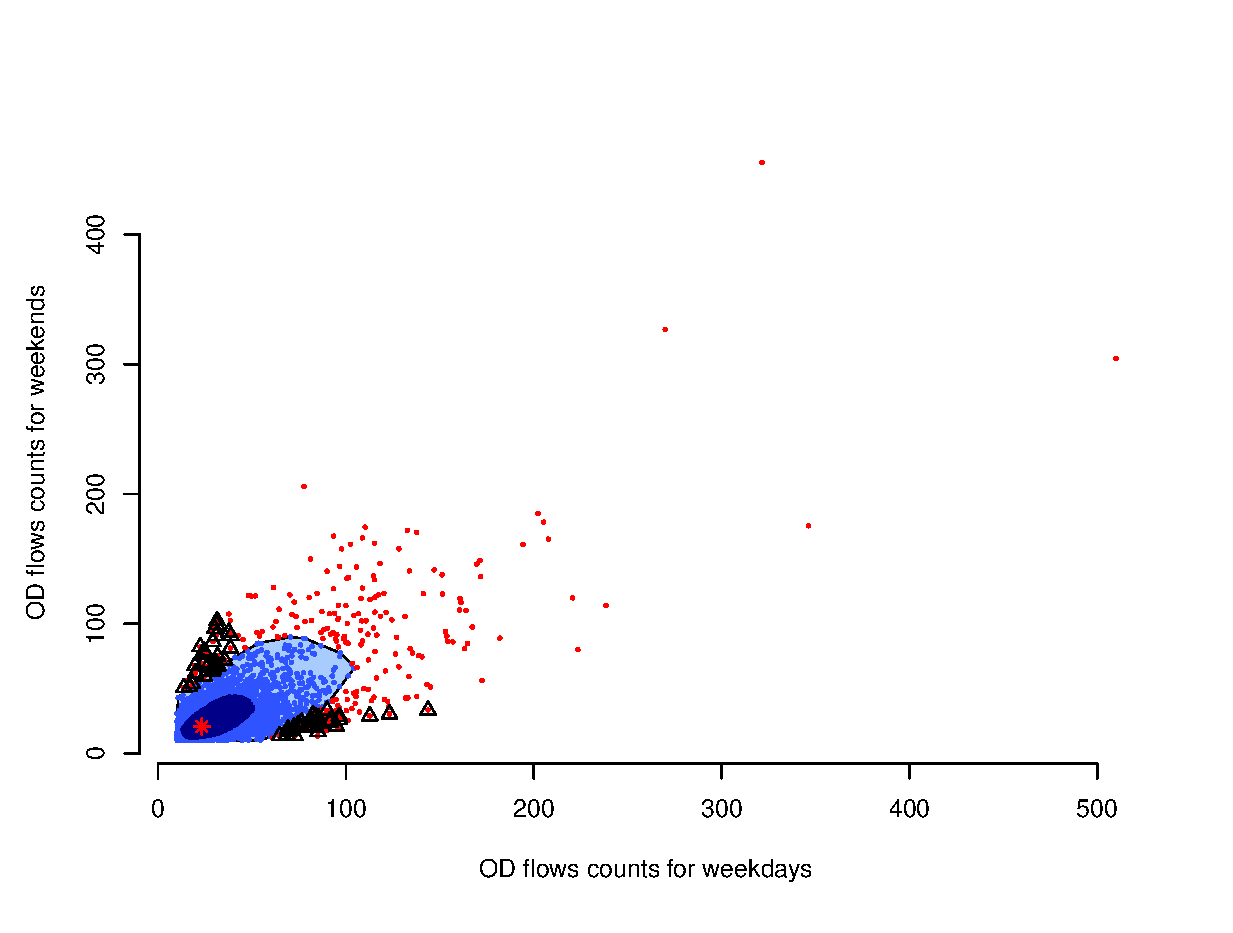
\includegraphics[width=\textwidth]{images/Outliers_rare_weekdays_weekends.eps}
		\caption{Relative OD flows outliers}
		\label{fig:weekdays_rare}
	\end{subfigure}
	\hfill %add desired spacing between images, e. g. ~, \quad, \qquad, \hfill etc. 	%(or a blank line to force the subfigure onto a new line)
	\begin{subfigure}[b]{0.49\textwidth}
		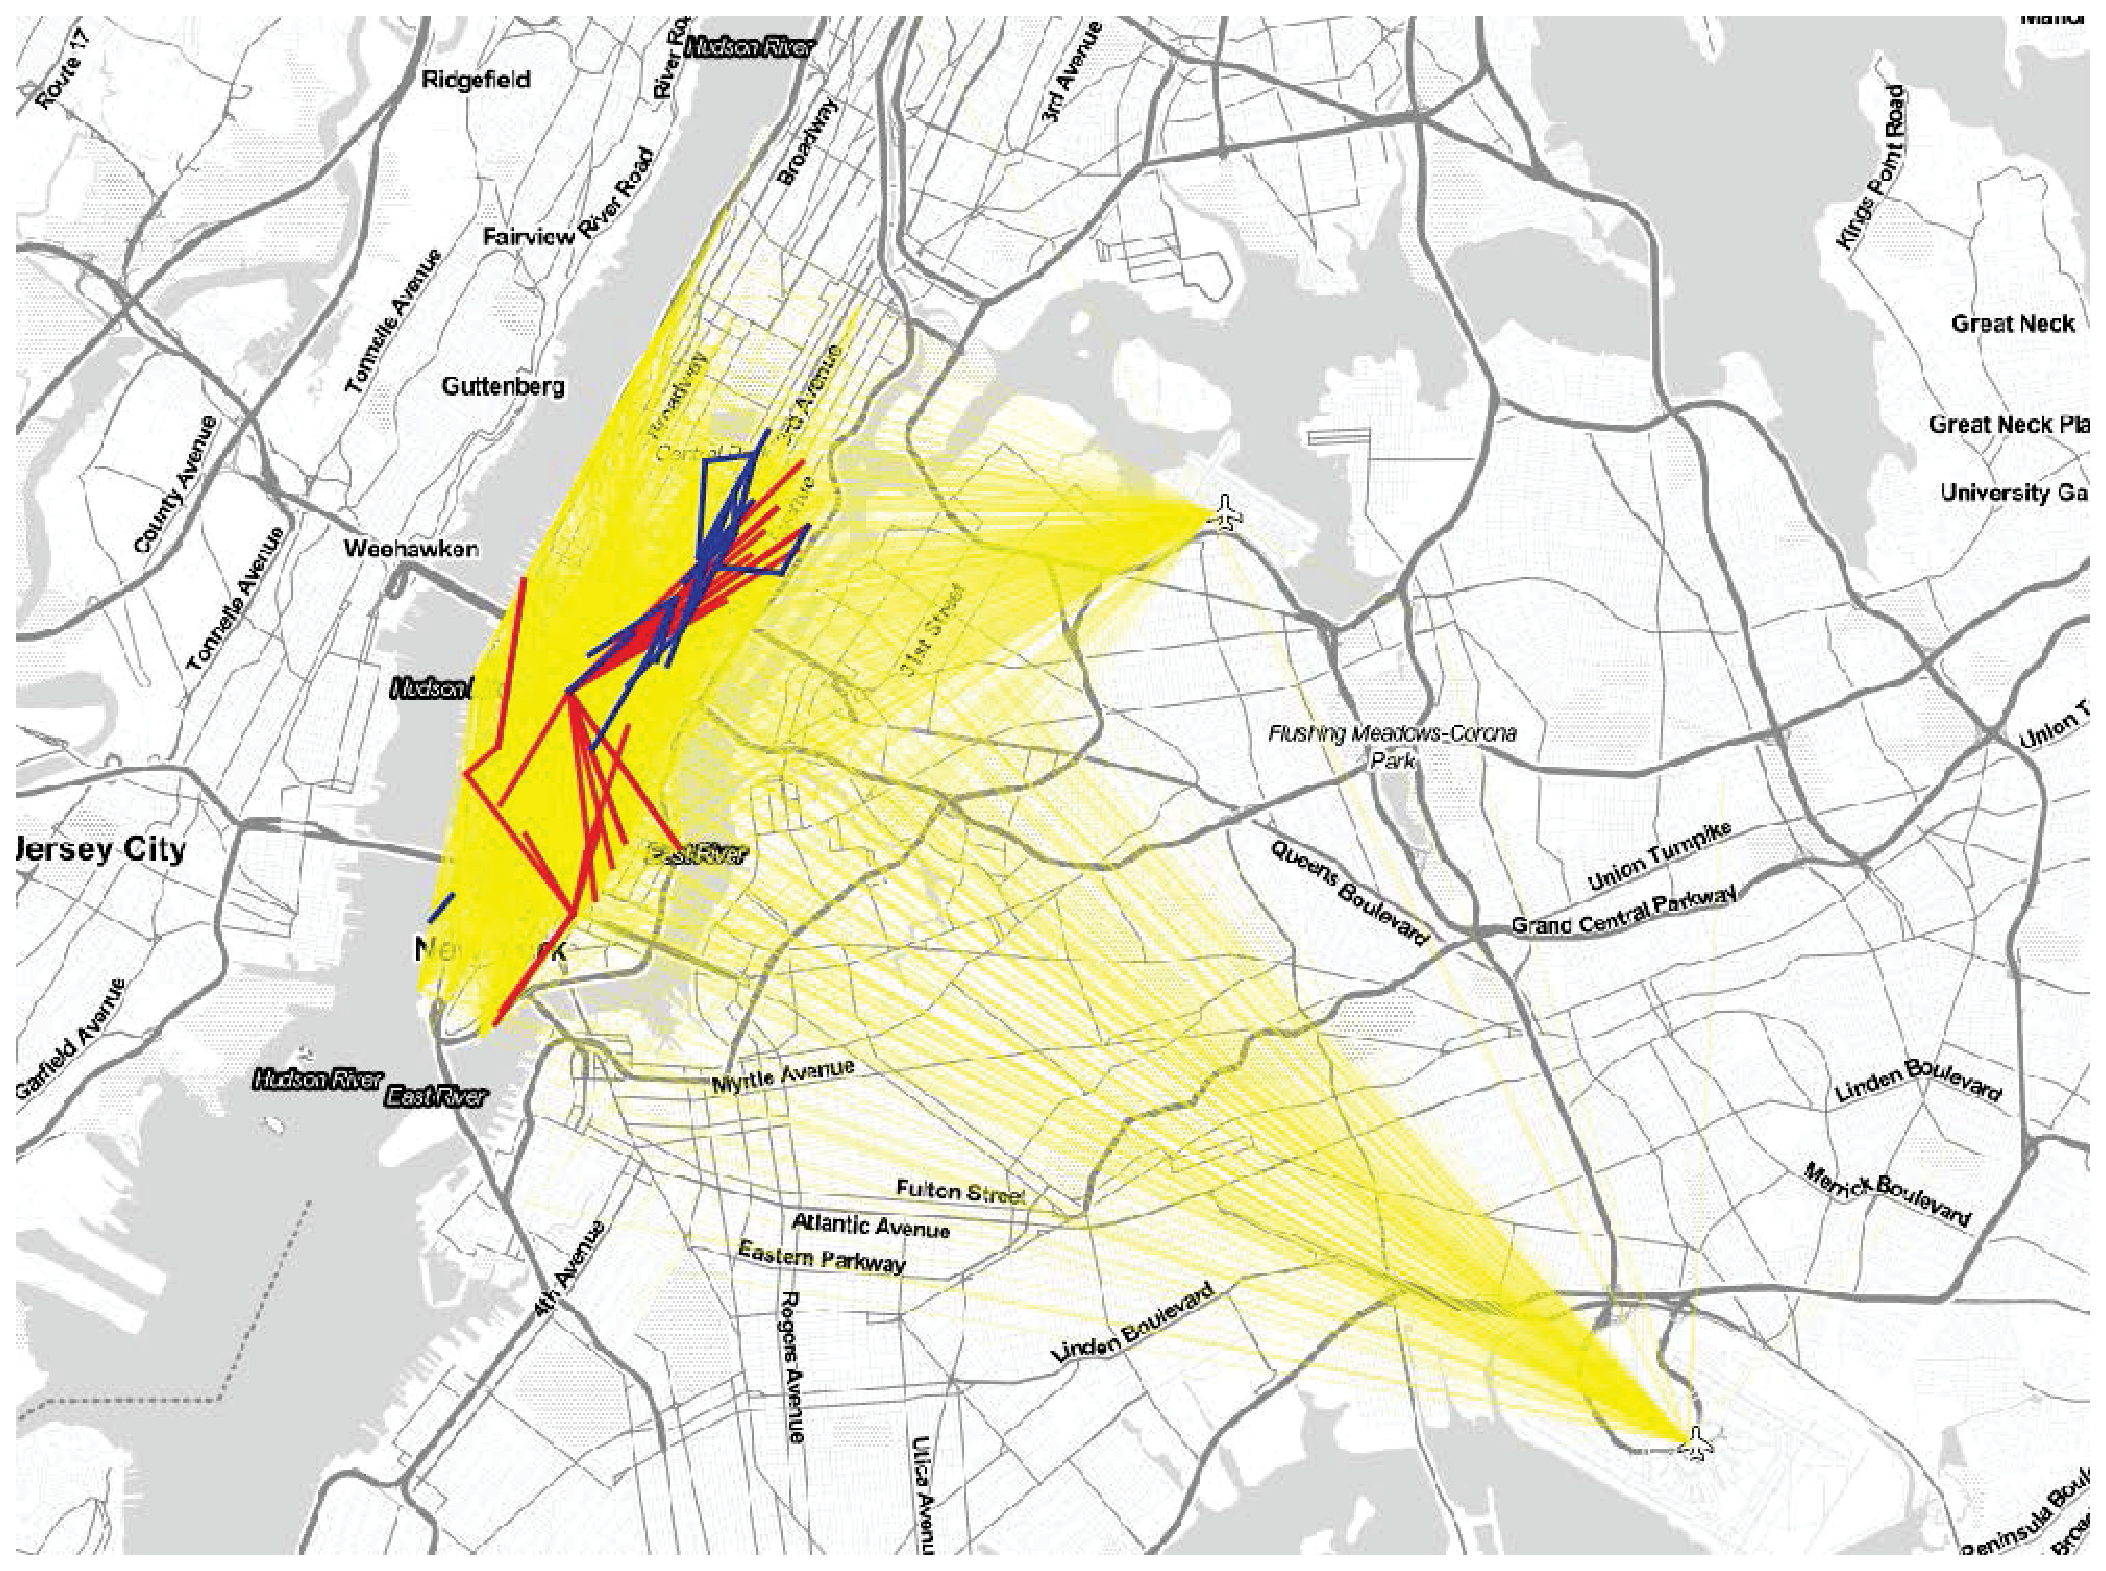
\includegraphics[width=\textwidth]{images/outliers_rare2_weekdays_weekends.eps}
		\caption{OD flow map for relative OD flows outliers}
		\label{fig:weekdays_rare_map}
	\end{subfigure}
	\caption{Relative OD flows outliers on weekdays and weekends: Triangles in Figure \ref{fig:weekdays_rare} coincide with red and blue lines in Figure \ref{fig:weekdays_rare_map}. }\label{fig:weekdays_rare_OD_map}	
\end{figure}

We also detected outlier OD flows using Mahalanobis distance.
The results are presented in Figure \ref{fig:week_ends_MD}. 
Far fewer outlier OD flows were detected using Mahalanobis distance than by the proposed approach.
The Mahalanobis method only considers the forward OD flows of the two datasets.
It identified OD flow outliers with high volume of trips because Mahalanobis distance considers the correlations between two OD flows.
Thus, Mahalanobis distance is more likely to identify outliers when two OD flows have large trip volumes.
In fact, the OD flows outliers from Mahalanobis distance are a subset of the outliers identified by the proposed method, as depicted in Figure \ref{fig:weekdays_high_map}.
Furthermore, the Mahalanobis distance approach could not detect the outliers detected by the proposed approach in Figure \ref{fig:weekdays_rare_OD_map} because the Mahalanobis distance approach cannot compare two flows to evaluate significant increases or decreases.


%DIF < which OD flows significantly decrease or increase by comparing two OD flows.
\DIFdelbegin %DIFDELCMD < 

%DIFDELCMD < %%%
\DIFdelend \begin{figure}
	\centering
	\begin{subfigure}[b]{0.49\textwidth}
		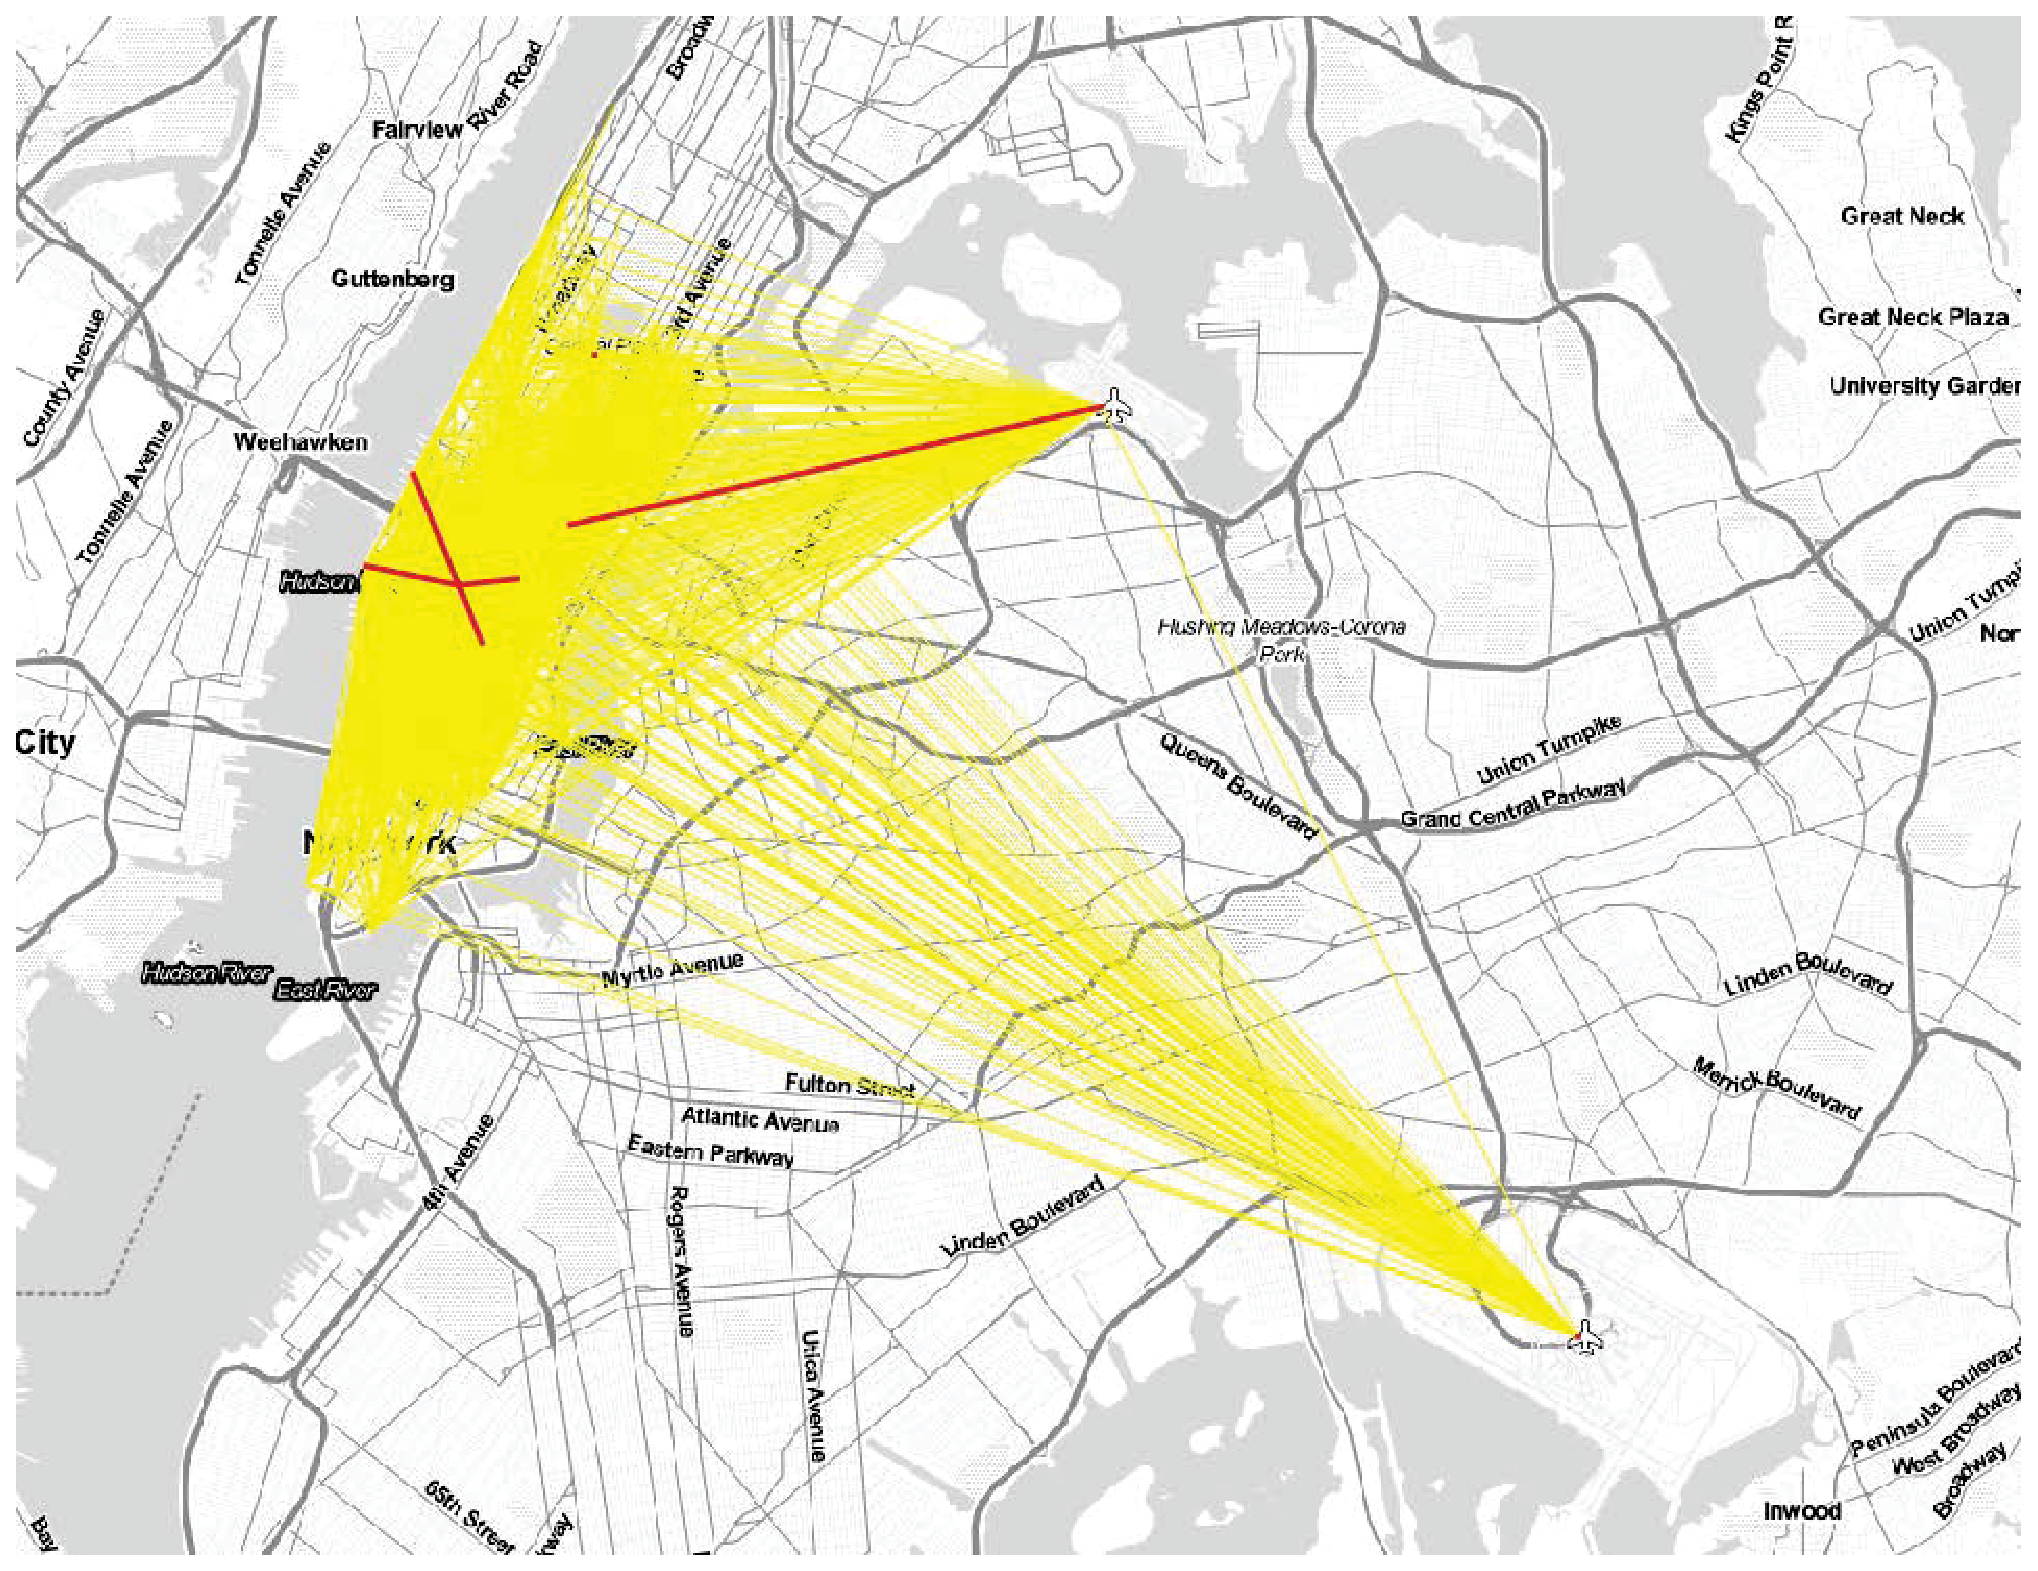
\includegraphics[width=\textwidth]{images/out_weekdays_weekends_md2_outlier.eps}
	\end{subfigure}
	\caption{Outlier OD flows on weekdays and weekends based on Mahalanobis distance. }\label{fig:week_ends_MD}	
\end{figure}

\subsubsection{Comparisons in scale}
We further investigated how two OD flows differ.
Our approach is sensitive to the difference in scale.
Hypothesis testing of \DIFaddbegin \DIFadd{the }\DIFaddend differences between two central regions in Figure \ref{fig:OD_comparisons} inadvertently revealed that the confidence interval was -0.0277 and 0.0157, which \DIFdelbegin \DIFdel{includes zero.
Thus, failing }\DIFdelend \DIFaddbegin \DIFadd{included zero.
Therefore, it failed }\DIFaddend to reject the null hypothesis\DIFdelbegin \DIFdel{. The }\DIFdelend \DIFaddbegin \DIFadd{, which indicated the }\DIFaddend two central regions were similar in terms of the spread.

\begin{figure}
	\centering
	\begin{subfigure}[b]{0.7\textwidth}
		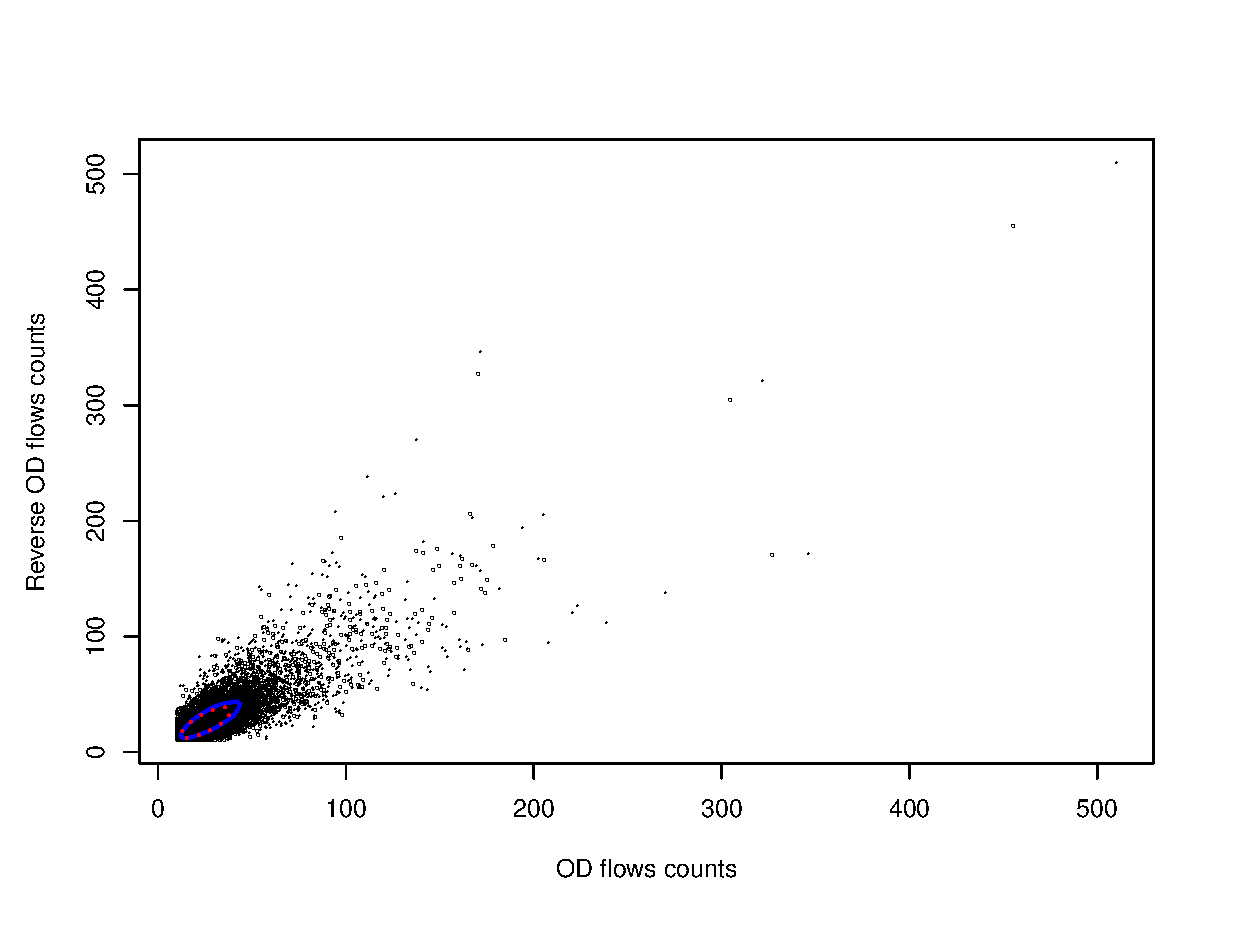
\includegraphics[width=\textwidth]{images/com_weekdays_weekends.eps}
	\end{subfigure}
	\caption{OD flows comparisons based on data depth: $\circ$ indicates the OD flows on weekdays and * indicates the OD flows on weekends; blue line presents the central region of the OD flows for the weekdays and red dotted line presents the central region of the OD flows on weekends. }\label{fig:OD_comparisons}	
\end{figure}

Interestingly, the standard statistic F-test was significant, $F(9530,7637) =1.1786$, $p \leq 0.05$.
The variances of two groups were significantly different. 
This result directly opposed that of the proposed approach.


%DIF < \subsection{Scalability}
%DIF < 
%DIF < \begin{figure}
%DIF < 	\centering
%DIF < 	\begin{subfigure}[b]{0.7\textwidth}
%DIF < 		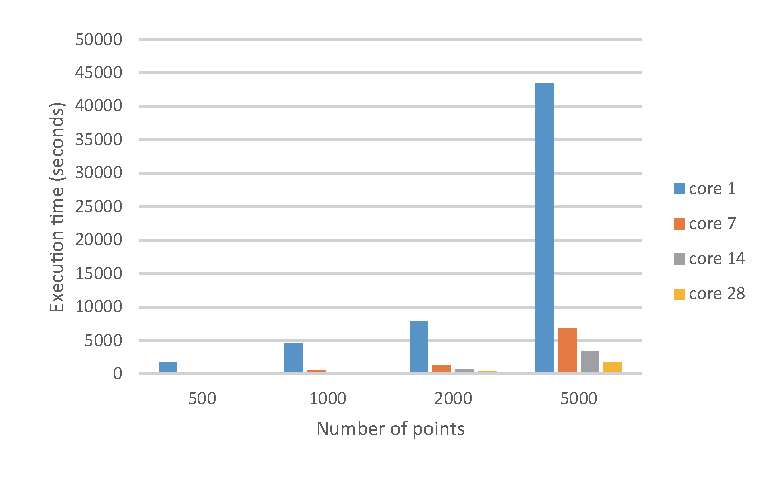
\includegraphics[width=\textwidth]{images/scalability.eps}
%DIF < 	\end{subfigure}
%DIF < 	\caption{Measure of time reduction. }\label{fig:scalability}	
%DIF < \end{figure}
\DIFdelbegin %DIFDELCMD < 

%DIFDELCMD < %%%
\DIFdelend \section{Discussion}
\label{sec:discussion}
The results demonstrate that the proposed method effectively identifies outlier OD flows based on data depth.
It is also possible to detect outlier OD flows by querying with conditional clauses, such as which outlier OD flows always have high trip volumes during time $t_1$ and time $t_2$.

As an alternative method, the state-of-the-art Mahalanobis \DIFdelbegin \DIFdel{distance }\DIFdelend \DIFaddbegin \DIFadd{distance-based }\DIFaddend approach detected similar outlier OD flows.
However, the number of outliers detected was different.
This occurred because our OD flows data had heavy tail distributions, that is, many of the OD flows with a long distance from the depth median depicted in Figure \ref{fig:weekdays_rare}. 
Mahalanobis distance is known to be inadequate when the underlying data have heavy \DIFdelbegin \DIFdel{tail }\DIFdelend \DIFaddbegin \DIFadd{tailed }\DIFaddend distributions \cite{wilcox12Book}. 
Thus, the presence of outliers may mask the detection of other outliers in Mahalanobis distance approach.
Furthermore, it can only detect OD flow outliers with high numbers of trips during time $t_1$ and time $t_2$. 
It is difficult to detect OD flows outliers that have different properties, such as substantial differences in the number of trips when comparing with time $t_1$ and time $t_2$.

In terms of the difference in spread, our approach used a bootstrap method to compare the central regions of data depth.
This approach investigated the difference in scale as well as the structure of data.
It can provide information how deeply points from group 1, OD flows at $t_1$, tend to be located within group 2, OD flows at $t_2$.
General statistics such as F-test only provide their difference in variation and do not further specify how groups differ. 

Interestingly, the F-test results revealed a statistically significant difference in terms of variation of OD flows on weekdays and weekends.
Our approach showed no statistically significant differences.
The difference may be caused by the sensitivity of F-test to non-normality \cite{Field12book}, which increases the Type-I error rate.
Conversely, data depth makes no assumptions about the distributions of the underlying dataset.


%DIF < when the sample size is large, small differences in group differences can produce a F test is significant. 
%DIF < 
%DIF < This F-test is known to be extremely sensitive to non-normality,
\DIFdelbegin %DIFDELCMD < 

%DIFDELCMD < %%%
\DIFdelend \section{Conclusions and Future Work}
\label{sec:conclusions}

This paper provides a new methodology for identifying outlier OD flows and \DIFaddbegin \DIFadd{detecting }\DIFaddend the difference in scale between two different OD flows at $t_1$ and $t_2$.
The proposed method is based on the concept of data depth.
Data depth is robust statistics, which is suited to \DIFaddbegin \DIFadd{datasets with the underlying distribution being }\DIFaddend non-Gaussian\DIFdelbegin \DIFdel{distribution of the underlying datasets}\DIFdelend .
Compared with standard statistics, this approach enhances understanding of the differences and the magnitude of the differences between \DIFdelbegin \DIFdel{tow }\DIFdelend \DIFaddbegin \DIFadd{two }\DIFaddend OD flows.


%DIF < adds different perspective how two OD flows differ and by how much. 
\DIFdelbegin %DIFDELCMD < 

%DIFDELCMD < %%%
\DIFdel{This }\DIFdelend \DIFaddbegin \DIFadd{The current }\DIFaddend study made no attempt to \DIFdelbegin \DIFdel{consider geographic contexts}\DIFdelend \DIFaddbegin \DIFadd{incorporate geographic contexts, }\DIFaddend such as locational circumstances or surrounding environment\DIFdelbegin \DIFdel{in understanding }\DIFdelend \DIFaddbegin \DIFadd{, in differentiating the }\DIFaddend OD flows. 
\DIFdelbegin \DIFdel{Ultimately, further investigation should }\DIFdelend \DIFaddbegin \DIFadd{Further investigations will }\DIFaddend focus on integrating the analysis of OD flows with geographic context.
Such an effort will lead to knowledge discovery and \DIFdelbegin \DIFdel{understanding the dynamics of urban flow.
}%DIFDELCMD < 

%DIFDELCMD < %%%
%DIF < 
%DIF < the bag gives an idea of the shape of the majority of the data cloud.
%DIF < how to generalize: point-based approach.
%DIF < 
%DIF < Tukey's depth makes no assumptions about the distribution from which observations are randomly sampled.  
%DIF < 
%DIF < 
%DIF < Outliers can be identified and treated in an interactive way.
%DIF < 
%DIF < Multivariate depth statistics are particularly suited to analyze non-
%DIF < Gaussian or, more general, non-elliptical distributions in Rd . Without
%DIF < In inference, tests for
%DIF < goodness of fit and homogeneity regarding location, scale and symmetry are based
%DIF < on depth statistics
%DIFDELCMD < 

%DIFDELCMD < %%%
%DIF < \subparagraph*{Acknowledgements.}
\DIFdelend \DIFaddbegin \DIFadd{better understandings regarding the dynamics in urban flows.
}\DIFaddend 


%%
%% Bibliography
%%

%% Please use bibtex, 

\bibliography{giscience2018}


\end{document}
